\documentclass [a4paper,normaltoc,normalfigtabnum, header, espacoumemeio, capchap, capsec, cappre, 12pt,notimes]{abntpoli}

\usepackage{xcolor}
\usepackage{graphicx}
\usepackage{acronym}
\usepackage[brazil]{babel}
\usepackage[T1]{fontenc}
\usepackage{amsmath}
\usepackage{amssymb}
\usepackage{listings}
\usepackage{tocbibind}
\usepackage[labelsep=endash, font=footnotesize]{caption}
\usepackage[alf, abnt-emphasize=bf]{abntcitepoli}
\usepackage[final]{listofsymbols}
\usepackage{url}
\usepackage{textcomp}
\usepackage{imakeidx}
\usepackage{subfig}
\usepackage[section]{placeins}
\usepackage{etoolbox}
\usepackage{dsfont} % fontes matem�ticas duplas como N, Z, R, para designar conjuntos
\usepackage[subfigure]{tocloft}
\usepackage[final]{pdfpages}

\usepackage{array}
\newcolumntype{L}[1]{>{\raggedright\let\newline\\\arraybackslash\hspace{0pt}}m{#1}}
\newcolumntype{C}[1]{>{\centering\let\newline\\\arraybackslash\hspace{0pt}}m{#1}}
\newcolumntype{R}[1]{>{\raggedleft\let\newline\\\arraybackslash\hspace{0pt}}m{#1}}

\renewcommand{\familydefault}{\sfdefault}

\makeindex[title=�ndice]


% 

\setcounter{lofdepth}{1}


\newlength\tablelen
\settowidth\tablelen{\tablename\;}
\addtolength\cfttabnumwidth{\tablelen}
\renewcommand\cfttabpresnum{\tablename\;}
\renewcommand\cfttabaftersnum{\,--\;}

\newlength\figlen
\settowidth\figlen{\figurename\;}
\addtolength\cftfignumwidth{\figlen}
\renewcommand\cftfigpresnum{\figurename\;}
\renewcommand\cftfigaftersnum{\,--\;}


\graphicspath{{./figuras/}}

\allowdisplaybreaks


   
   %\lhead{\thechapter}
   
   

\begin{document}
	\pagenumbering{roman}
	
	
\autor{Pablo Alejandro de Abreu Urbizag�stegui}
\titulo{Modelagem de C�lulas de Renshaw e Sua Utiliza��o em Simula��es do Sistema Neuromuscular.}
\orientador{Andr� Fabio Kohn}
\local{S�o Paulo}
\areadeconcentracao{Engenharia Biom�dica}
 \comentario{Disserta��o apresentada � Escola Polit�cnica da \mbox{Universidade} de S�o Paulo para a obten��o do t�tulo de Mestre em Ci�ncias}
\data{2018}
\capa
\folhaderosto

	%\pretextualchapter{Agradecimentos}

Primeiramente, agrade�o ao Prof. ....

Aos colegas ...

Aos meus pais ....

....

Por fim, � quem me financiou.
	
	%\newpage
	%\begin{resumo}
\noindent Urbizagastegui, Pablo Alejandro de Abreu.
\textbf{Modelagem de c�lulas de Renshaw e sua utiliza��o
em simula��es do sistema neuromuscular}.
2019. 98 f. Disserta��o (Mestrado) - Escola Polit�cnica,
Universidade de S�o Paulo, S�o Paulo, 2019. \\
\\
%As C�lulas de Renshaw s�o interneur�nios inibit�rios localizados na
%medula espinhal se mam�feros como gatos, ratos e seres humanos. Por
%desempenharem um papel central no circuito de inibi��o recorrente,
%acredita-se que as c�lulas de Renshaw sejam importantes para a gera��o
%e coordena��o de atividades musculares. Entretanto, at� hoje n�o se sabe
%qual a fun��o principal desse neur�nio.
O objetivo principal
desse trabalho foi realizar um estudo computacional sobre as influ�ncias
da c�lula de Renshaw sobre motoneur�nios em diferentes situa��es, mas
tamb�m envolveu parametriza��es e recomenda��es de t�cnicas para melhorar
o desempenho do sistema de simula��o utilizado.
O ajuste de par�metros e as simula��es foram guiados por
dados experimentais de gatos dispon�veis na literatura.
Os resultados obtidos, al�m de mostrar que o modelo utilizado
foi capaz de reproduzir de forma satisfat�ria v�rias observa��es experimentais,
sugerem que as c�lulas de Renshaw podem afetar a for�a muscular gerada
e a taxa de disparos e o recrutamento de motoneur�nios.
Dentre as simula��es e an�lises realizadas, destacam-se os fatos de que,
quando as c�lulas de Renshaw estava presentes, houve maior tend�ncia a
ocorrer invers�es na ordem de recrutamento, maior velocidade no
desenvolvimento da for�a muscular e a capacidade de diminuir oscila��es
em 10 Hz por meio de cancelamento de fases.
O modelo foi disponibilizado como uma ferramenta \textit{open source},
facilitando a reproduzibilidade e extens�o dos assuntos abordados.

\noindent Palavras-chave: C�lula de Renshaw. Neur�nios motores.
Neurofisiologia. Simula��o.
\end{resumo}

\begin{abstract}

\noindent Urbizagastegui, Pablo Alejandro de Abreu.
\textbf{Modelling of Renshaw cells and its utilization in simulations of the
neuromuscular system}.
2019. 98 f. Disserta��o (Mestrado) - Escola Polit�cnica,
Universidade de S�o Paulo, S�o Paulo, 2019. \\
\\
The present work carries out a computational study on
the influences of Renshaw cell on motoneurons in different situations,
but also involves parametrization and recommendations of techniques
to improve the performance of the simulation system utilized. The
adjustments of parameters and simulations were guided by cat experimental
data available in the literature. The results obtained not only showed
that the model used could properly reproduce several experimental
observations, but also suggested that Renshaw cells can affect muscle
strength and motoneuronal rate and recruitment. Among the simulations
and analyzes performed, it should be emphasized that when the Renshaw
cells were included there was a greater tendency for inversions in the
orderly recruitment of motoneurons to occur, greater speed of muscle force
development and decrease of oscillations at 10 Hz by phase cancellation.
The model was distributed as an open source tool, facilitating the
reproducibility and extension of the observations described.

\noindent Keywords: Renshaw cell. Motoneurons. Neurophysiology. Simulation.
\end{abstract}

	
%	\renewcommand\listfigurename{Lista de Figuras}
	
	\listadefiguras
	\listadetabelas
	\renewcommand\symheadingname{Lista de S�mbolos}
\renewcommand\symheading{\pretextualchapter{Lista de S�mbolos}}

\opensymdef
	\newsym[S�mbolo 1]{A}{\alpha}
	\newsym[S�mbolo 2]{X}{x}	
\closesymdef


	\listofsymbols	
	%\lhead{\thechapter}
	%%% modifica a maneira de apresentar a lista de siglas
	\def\bflabel#1{{{\textsf{#1}}\hfill}}
	\renewenvironment{AC@deflist}[1]%
	      {\if AC@nolist%
		\else%
		    \raggedright\begin{list}{}%
		    {\settowidth{\labelwidth}{\textsf{#1}+8pt}%
		    \setlength{\leftmargin}{\labelwidth}%
		    \setlength{\itemsep}{0.5pt}%
		    \addtolength{\leftmargin}{\labelsep}%
		    \renewcommand{\makelabel}{\bflabel}}%
		 \fi}%
		{\if AC@nolist%
		  \else%
		    \end{list}%
		\fi}%

\pretextualchapter{Lista de Siglas}

\begin{acronym}[NARMAX]
    \acro{SNC}[SNC]{Sistema Nervoso Central}
    \acro{MN}[MN]{Motoneur�nio}
    \acro{IN}[IN]{Interneur�nio}
    \acro{ACh}[ACh]{Acetilcolina}
    \acro{PEPS}[PEPS]{Potencial Excitat�rio P�s Sin�ptico}
    \acro{EMG}[EMG]{Eletromiografia}
    \acro{CVM}[CVM]{Contra��o Volunt�ria M�xima}
    \acro{FF}[FF]{Fast Fatiguing}
    \acro{FR}[FR]{Fast Fatigue Resistant}
    \acro{S}[S]{Slow}
    \acro{CR}[CR]{C�lula de Renshaw}
    \acro{PIPS}[PIPS]{Potencial Inibit�rio P�s Sin�ptico}
    \acro{AHP}[AHP]{Afterhyperpolarization}
    \acro{FxI}[FxI]{frequ�ncia de disparo \textit{versus} corrente injetada}
\end{acronym}

	
	\sumario	
	
	%\pagestyle{fancyplain}
	\chapter{Introdu��o}
\label{cap:intro}

O objetivo desse trabalho � estudar as C�lulas de Renshaw e suas fun��es 
usando modelos computacionais realistas. A maioria dos dados usados aqui v�m
de experimentos realizados em membros inferiores de gatos. Como esse tipo de
experimento raramente � realizado hoje em dia, esses dados atualmente s�o
obtidos de ratos. Dessa forma, dados de ratos ser�o usados com cautela, com 
o devido aviso.
%The goal of the present work is to study the Renshaw cells and its functions
%using realistic computational models. Most of the data used here comes from
%experiments carried out on the cat hindlimb. As cat experiments are seldom
%performed nowadays, most of the recent data on the Renshaw cells come from 
%rat. Therefore, rat data will be used with caution and expressly indicated.

\section{O Sistema Motor}
O \textbf{Sistema Nervoso Central} � composto pelo c�rebro e pela 
\textbf{coluna espinhal}. O segundo � subdividido em cervical, tor�cico,
lombar e sacral, sendo cada um desses divididos em v�rios segmentos. A
coluna espinhal recebe e processa informa��o de m�sculos, articula��es e pele
e controla movimentos. Nesse contexto, o termo \textbf{aferente} � usado para
identificar sinais chegando � coluna espinhal, enquanto sinais entregues aos
m�sculos s�o chamados de \textbf{eferentes} \cite{kandel13}.
%The \textbf{central nervous system} (CNS) comprises the brain and the
%\textbf{spinal cord} (SC).
%The latter is further subdivided into cervical, thoracic, lumbar, and sacral,
%where each of these regions contains several segments.
%The SC receives and processes information from muscles, joints, and skin and 
%controls movement. In this context, the term \textbf{afferent} is used to
%identify
%the signals reaching the SC, whereas signals delivered to muscles are named
%\textbf{efferent} \cite{kandel13}.


O tipo de m�sculo estudado aqui � o \textbf{m�sculo esquel�tico}, que �
respons�vel por movimentar os ossos, olhos, inala��o e exala��o, controlar
express�es faciais e fala \cite{bear16}. Movimentos que diminuem o �ngulo
entre um segmento e seu segmento proximal s�o chamados de flex�o,
enquanto movimentos que aumentam esse �ngulo s�o chamados de
extens�o \cite{oxford}. Sendo assim, m�sculos podem ser
classificados como \textbf{flexores} e \textbf{extensores}. Se eles t�m a 
mesma fun��o, s�o chamados de \textbf{sinergistas} um do outro. Por outro
lado, se puxam a articula��o para lados opostos, s�o chamados de
\textbf{antagonistas} \cite{bear16}.
%The type of muscle studied herein is the \textbf{skeletal muscle}, which
%functions to move bones around joints, eyes within the head,
%inhalation/exhalation, control facial expression, and speech \cite{bear16}.
%Movements that decrease the angle between a segment and its proximal segment are
%described as flexion, whereas movements that increase it are called extension
%\cite{oxford}. Therefore, muscles can be classified as 
%\textbf{flexors} and \textbf{extensors}. If muscles work together, they are
%called
%\textbf{synergists} of one another. If they pull a joint on the opposite
%direction, they are called \textbf{antagonists} to one another \cite{bear16}.

Em cada m�sculo esquel�tico existem centenas de fibras musculares. Elas s�o
importantes n�o somente para a gera��o de for�a, mas tamb�m para
\textbf{propriocep��o}, j� que o \textbf{fuso muscular}, que consiste em
v�rias fibras esquel�ticas especializadas contidas em umas c�psula fibrosa,
fornece informa��o sobre o comprimento do m�sculo.
%Within each skeletal muscle there are hundreds of muscle fibers. They are
%important not only for force generation, but also for \textbf{proprioception},
%since the \textbf{muscle spindle}, which consists of several types of specialzed
%skeletal muscle fibers contained in a fibrous capsule, provides feedback about
%muscle length.

\section{A Circuitaria da Coluna Espinhal}
Um corte transversal da coluna espinhal � mostrado na Figura \ref{fig:ce}. O
n�cleo central � a \textbf{mat�ria cinzenta}, que cont�m o corpo de c�lulas
nervosas. A \textbf{subst�ncia branca} em volta dessa regi�o � abriga ax�nios
ascendentes e descendentes. A subst�ncia cinza ainda � subdividida em
\textbf{corno ventral} e \textbf{corno dorsal}.
%A cross section of the SC is shown in
%Fig. \ref{fig:sc}. The central core is the
%\textbf{gray matter}, which contains nerve cell bodies. The surrounding
%\textbf{white matter}
%accommodates ascending and descending axons.
%The gray matter is further subdivided in \textbf{ventral} and
%\textbf{dorsal horns}.

% TODO edit figure
\begin{figure}[ht!]
	\center
	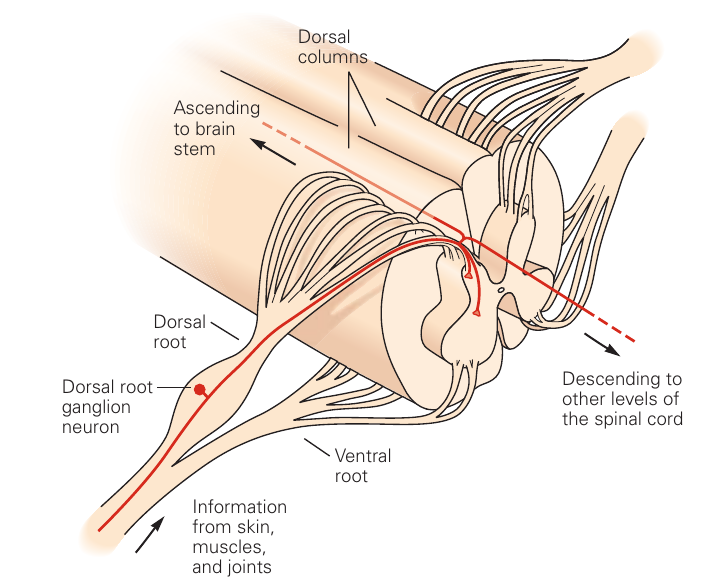
\includegraphics[scale=0.6]{sc.png}
	\caption{Vis�o da sess�o transversal da coluna espinhal
        [Adaptado de Kandel (2013)].}
	\label{fig:ce}
\end{figure}

O corno ventral cont�m tipos especializados de neur�nios: o
\textbf{motoneur�nio} (MN), que possui \textbf{ax�nios motores} inervando
m�sculos espec�ficos, e o \textbf{interneur�nio} (IN), que est� envolvido em
v�rios circuitos neuronais, seja no n�vel do segmento ou conectando com
estruturas de n�veis superiores. O conjunto de um MN, seu ax�nio e todas as
fibras musculares que este inerva � chamado de \textbf{unidade motora}
\cite{liddell25,sherrington25}.

%The ventral
%horn contains specialized types of neurons: the \textbf{motor neurons} (MNs),
%which have \textbf{motor axons} innervating specific muscles, and the
%\textbf{interneurons}
%(INs), which
%are involved in many neural circuits either at the segmental level or connecting 
%with upper level neural structures.
%The collection of one MN, its axon and all the muscle fibers it innervates is
%called a \textbf{motor unit} (MN) \cite{liddell25,sherrington25}.

A raiz dorsal consiste em fibras nervosas aferentes que carregam informa��es
dos m�sculos, tend�es, articula��es e pele para a coluna espinal, enquanto que
a raiz ventral, por sua vez, consiste em ax�nios inervando m�sculos e fusos
musculares. Existem duas categorias de MN: alfa (MN$\alpha$) e gama
(MN$\gamma$). O primeiro inicia diretamente as contra��es de fibras musculares.
O conjunto de MNs$\alpha$ que ineram um �nico m�sculo � chamado de
\textbf{n�cleo motor} ou \textbf{pool de MN}. N�cleos motores formam colunas
que percorrem o comprimento da coluna espinhal \cite{kandel13,bear16}.
%The dorsal root
%consists of
%afferent nerve fibers that carry information from muscles, tendons, joints and
%the skin into the spinal cord,
%whereas the ventral root, on the other hand, comprises axons innervating muscles
%and muscle spindles.
%There are two categories of MN: alpha ($\alpha$) and gamma ($\gamma$).The former
%directly
%initiates contractions of a muscle fibers. The collection of $\alpha$MNs that
%innervate a single muscle is called a \textbf{motor nucleus} or \textbf{MN pool},
%and motor nuclei form columns that run the length of the spinal cord
%\cite{kandel13,bear16}.

As termina��es dos ax�nios motores inervando um m�sculo se separam em diversos
ramos e formam incha�os chamados de \textbf{bot�es sin�pticos}, de onde os MNs
liberam o neurotransmissor acetilcolina (ACh). Cada bot�o � posicionado sobre
uma regi�o especializado da membrana muscular contendo uma alta densidade de
receptores de ACh nicot�nico. Como resultado, ACh liberada dos terminais dos
ax�nios motores interagem com esses receptores para produzir um
\textbf{potencial excitat�rio p�s sin�ptico} (PEPS) \cite{kandel13}.
%The endings of motor axons innervating a muscle split into several fine branches
%and form swellings called \textbf{synaptic boutons}, from which the MN releases
%the neurotransmitter acetylcholine (ACh). Each bouton is positioned over a 
%specialized region of the muscle membrane containing a high density of nicotic
%type of ACh receptor. As a result, ACh released from motor axon terminals
%interact with ACh receptors to produce an excitatory postsynaptic potential
%(EPSP)\cite{kandel13}.

O MN$\alpha$ � subdividido em diferentes tipos dependendo das propriedades dos
pr�prios neur�nios e das fibras musculares que eles inervam: contra��o r�pida
e fadiga r�pida (do ingl�s \textit{fast, fatiguing}, FF); contra��o r�pida e
resistente � fadiga (do ingl�s \textit{fast,fatigue resistant}, FR); e lenta
(do ingl�s \textit{slow}, S).% TODO ref and enoka obs and pool not homogeneous
%% bear p 461, try to write it properly (fiber type and MU type)
%The $\alpha$MN are further subdivided into different types depending on the
%properties of the neurons themselves and the muscle fibers they innervate:
%fast, fatiguing (FF); fast, fatigue resistant (FR); and slow (S). 

% TODO anatomy figure of SC? (p 828)

\section{As C�lulas de Renshaw}
A \textbf{C�lula de Renshaw} (CR) � um IN localizado na corno ventral da coluna
espinhal, medial �s colunas de motoneur�nios. Suas ramifica��es axonais se
espalham por dist�ncias maiores que 12mm rostralmente ou caudalmente
\cite{jankowska71,jankowska73} e faz sinapses com uma variedade de neur�nios.
%The \textbf{Renshaw Cell} (RC) is an IN located at the ventral horn of the
%spinal cord, medial to the motorneuronal columns. Its axon branchings spread over
%distances
%greater than 12mm rostrally or caudally \cite{jankowska71,jankowska73} and target a variety
%of neurons.

A exist�ncia da CR foi descrita pela primeira vez em 1941 por Birdsey Renshaw
\cite{renshaw41} em um experimento com animais com as respectivas ra�zes
dorsais seccionadas cirurgicamente, quando foi demonstrado que que uma
estimula��o antidr�mica de ax�nios motores causavam um inibi��o de MNs$\alpha$
inervando os mesmos m�sculos (ou \textbf{hom�nimos}) e os m�sculos sinergistas.
Mais tarde, foi mostrado que essa inibi��o � mediada por meio de ramos
colaterais de ax�nios motores fornecendo entradas sin�pticas excitat�rias para
CRs, que por sua vez inibem diversos MNs que inervam o respectivo m�sculo
\cite{eccles54}.
%The existence of the RC was first described in 1941 by Birdsey Renshaw
%\cite{renshaw41} in an experiment in animals with the respective
%dorsal root sectioned surgically, demonstrating that an
%antidromic stimulation of motor axons caused an inhibition of
%$\alpha$MNs
%innervating the same (or \textbf{homonymous}) and synergistic muscles. Later, it was shown that this
%inhibition is mediated through motor axon collaterals delivering excitatory synaptic inputs to
%RCs, which in turn inhibit several MNs that innervate the respective muscle
%\cite{eccles54}.

% TODO Figure with main connections and explaining

Pode-se perceber que essa rede de neur�nios cont�m um circuito disin�ptica que
come�a e termina no mesmo neur�nio: um MN excita uma CR, que por sua vez inibe
os MNs hom�nimos. Essa situa��o, em que um n�cleo motor inibe a si mesmo por
meio de algum IN inibit�rio, � conhecida como uma \textbf{inibi��o recorrente}.
Outros elementos envolvidos nesse esquema tamb�m recebem esse termo, como, por
exemplo, ramos colaterais recorrentes e potencial inibit�rio p�s sin�ptico
(PIPS) recorrente.
%As one can see, this neural network contains a disynaptic pathway that starts
%and ends at the same neuron: a MN provides an excitatory input to a RC, which in
%turn provide inhibitory input to the homonymous MN. This spinal pathway provides
%an inhibition known as \textbf{recurrent inhibition}. Other elements involved
%on this scheme also receive this label, such as recurrent axon collaterals
%and recurrent inhibitory postsynaptic potentials (IPSPs).

% TODO The connections shown is Figure ___ is a simplified view.
% unidirectional MN-RC connections, MN synapses on RC (hultborn88), RC synapses
% on MN (Fyffe 91)

\subsection{Entradas das C�lulas de Renshaw}
\subsubsection{De MNs$\alpha$}
Ativa��es de CRs s�o obtidas de estimula��es de v�rios nervos e aumentam
gradativamente com o acr�scimo de intensidade de estimula��o de nervos
individuais, sugerindo que uma �nica CR � excitada por ramos colaterais de
v�rios MNs \cite{eccles54,eccles61b}. Esses colaterais recorrentes se espalham
por uma dist�ncia de n�o mais do que 1 mm dos seus corpos celulares de origem
e possuem a maioria de seus bot�es sin�pticos convergindo para a �rea onde as
CRs est�o localizadas \cite{cullheim78}. Essa caracter�stica mostra que
excita��es podem ser obtidas somente de n�cleos motores localizados na
vizinhan�a de determinada CR e, portanto, depende da proximidade entre os
neur�nios. Al�m disso, como alguns n�cleos motores podem alcan�ar dist�ncias de
10 mm, apenas uma parte de um n�cleo motor pode se projetar para determinada
CR \cite{romanes51,burke77}.
%Activation of RCs are obtained from stimulation of several nerves and smoothly
%increase with increasing intensity of stimulation of individual nerves,
%suggesting that a single RC is excited by axon collaterals of many MNs 
%\cite{eccles54,eccles61b}. These
%recurrent collaterals spread a distance of no more than 1 mm from their parent
%cell body and have the majority of their synaptic boutons converging to
%the area where the RCs are located \cite{cullheim78}. This caracteristic shows 
%that excitation can be obtained only from motor nuclei located in the
%neighbourhood of a given RC and is
%therefore based on proximity factors. Furthermore, since some motor
%nuclei can be as long as 10 mm, only part of a motor nucleus may project to a 
%given RC \cite{romanes51,burke77}.

Al�m de depender de dist�ncias, converg�ncia para CRs tamb�m s�o baseadas em
fatores funcionais. Essa ideia � sustentada por evid�ncias mostrando que CRs
s�o excitadas principalmente por MNs de m�sculos sinergistas e n�o por aqueles
estritamente antagonistas \cite{ryall72,eccles61b}.
%Besides proximity factors, converge to RCs are also based on functional factors.
%This is supported by evidences showing that RCs are excited mainly by MNs 
%of synergistic muscles and not by those of strict antagonists
%\cite{ryall72,eccles61b}.

Nota-se que nem todos os MNs d�o origem a colaterais recorrentes. Apesar de
sempre estarem presentes em MNs inervando m�sculos do tornozelo e do joelho,
eles est�o ausentes em MNs de m�sculos curtos plantares do p�
\cite{cullheim78}.
%It should be noted that not all MNs give off recurrent collaterals.
%Despite always being given off by MNs innervating ankle and knee muscles, they
%are absent in MNs of short plantar foot muscles \cite{cullheim78}.

\subsubsection{De Vias Aferentes}
Outra via de ativa��o descrita na literatura � a excita��o e inibi��o
polissin�ptica ocasionada pela estimula��o de aferentes cut�neos, ra�zes
dorsais, fibras aferentes ipsilaterais dos grupos II e III e aferentes
contralaterais de alto limiar \cite{baldissera11}.

\subsubsection{De Vias Descendentes}
As CRs est�o podem apresentar efeitos inibit�rios e/ou excitat�rios quando
est�mulos el�tricos s�o aplicados em alguns centros supra espinhais, como o
c�rtex cerebral \cite{maclean67}, o n�cleo vestibular \cite{pompeiano85}, o
t�lamo \cite{maclean67}, entre outros. Esses efeitos podem se expressar direta
ou indiretamente por meio dos MNs $\alpha$.


\subsection{Sa�das das C�lulas de Renshaw}
\subsubsection{Para MNs $\gamma$}
Os MNs $\gamma$ do tipo est�tico e din�mico recebem inibi��o recorrente das
CRs \cite{ellaway81,appelberg83}.

Vale ressaltar que MNs $\gamma$ apenas ocasionalmente d�o origem a ramos
colaterais recorrentes e n�o parecem ser de grande influ�ncia na ativa��o das
CRs \cite{westbury82,granit57,kato74}, sugerindo, assim, que MNs $\gamma$
recebem inibi��o recorrente via CR predominantemente por meio de MNs $\alpha$
\cite{ellaway81,appelberg83}.

% TODO RC functions

\section{Distribui��o do Potencial Inibit�rio P�s Sin�ptico Recorrente}

\subsection{Outputs from Renshaw Cells}
% TODO distribution of IPSPs, here and later? There must be more to it
% (McCurdy&Hamm94) "altough these studies uniformly report that recurrent
% inhibition is found between MNs innervationg muscles that have disparate
% mechanical actions, recurrent inhibition is not found between motor pools 
% that innervate direct antagonists at a joint" - I don't quite understand that

Recurrent inhibition is evoked in a number of motor nuclei after the stimulation
of the MNs of a given muscle. The recurrent IPSPs in the homonymous MNs are found
to be larger, but many other MNs are also strongly inhibitied
\cite{eccles54,eccles61b}.
% Windhorst 90, sec. 5, 2 (1)
\subsection{Aspectos Topogr�ficos}

\subsection{Aspectos Funcionais}

% TODO RC functions

% \section{Renshaw Cells Characteristics}?

\section{ReMoto}
% TODO why exactly am I using a computational model here?
As shown previously, the RI circuit is considerably complex and is believed to
have important functions on the final output delivered to muscles. Despite all of
the efforts to comprehend the role of the RC on this network, 

% TODO there many other uses... maybe put the ones useful for me
On this aspect, a computational model can be very useful. It can be used to make
predictions, test theories or provide insights to experimentation. In the case of
the complex RI circuit, it might shed light over 



\index{problema}
O problema que esta tese aborda .... 

Algo importante a saber ao escrever em portugu�s � que os arquivos .tex devem ser salvos com decodifica��o ISO 8859-15.

\section{Objetivos}
\index{objetivos}
\index{exemplo! sigla}
O objetivo central do trabalho apresentado, realizado na \ac{USP} (este foi um exemplo de uso de sigla),  � ...


\section{Estrutura do texto}

\index{estrutura}
Este texto est� organizado da seguinte maneira ... 




	\chapter{Objetivos}
\section{Melhora de desempenho}
O tempo de execu��o de uma simula��o se torna um 
fator limitante quando se deseja estudar sistemas mais complexos. Sendo assim,
um dos objetivos desse trabalho � melhorar o desempenho computacional do
simulador. 
Vale ressaltar que esse n�o � o foco principal, pois esse tipo de
desenvolvimento pode ser bastante complexo e demorado por si s�.

\section{Avalia��o e valida��o do circuito de inibi��o recorrente}
Outro objetivo deste trabalho � reparametrizar e validar
o modelo das
CRs em n�veis de neur�nios e de redes de neur�nios, analisando se os
resultados s�o consistentes com dados fisiol�gicos de gatos.

\section{Estudo explorat�rio sobre o circuito de inibi��o recorrente}
Como �ltimo objetivo, deseja-se realizar um estudo explorat�rio para
entender como o modelo parametrizado se comporta 
em diferentes situa��es, algumas das quais se basearam em trabalhos
experimentais e computacionais.

 	\chapter{Metodologia}
Em todas as simula��es descritas a seguir, foi utilizado o m�todo de 
integra��o num�rica de Runge-Kutta de quarta ordem e com passo de
integra��o de 0.05 ms. Os dados obtidos podem ser acessados por meio
do link: https://dx.doi.org/10.17605/OSF.IO/QNMBH. Os c�digos
desenvolvidos para realizar as simula��es e processar os resultados,
por sua vez, podem ser encontrados no GitHub:
https://github.com/pabloabur/projectFR/tree/masters.

\section{Desempenho computacional}
Tr�s abordagens distintas ser�o consideradas nessa parte: A utiliza��o de um 
\textit{cluster}, Python na sua implementa��o original (CPython) e Cython.
As medi��es do tempo de execu��o, realizadas por meio da biblioteca \textit{time},
levar�o em conta apenas os trechos do c�digo
que se repetem v�rias vezes e que, consequentemente, cont�m os maiores
``gargalos'' na simula��o.

\subsection{Cluster �guia}
O \textit{cluster} �guia � composto por 64 servidores f�sicos com 20 \textit{cores} e 
512 GB de RAM. Seu processador � um Intel(R) Xeon(R) CPU E7-2870 com 2.4 GHz.
A vers�o do Python dispon�vel para utiliza��o nesse sistema � 2.7.13, da
distribui��o Anaconda2 4.4.0.

Primeiramente, o uso de ferramentas para passagem de mensagens em um sistema
distribu�do ser� analisado para simula��es simples, com uma corrente injetada
de 10 nA no soma de MNs. O c�lculo da for�a gerada tamb�m ser� computado.
Para esse fim, o pacote
Python MPI4Py, que possibilita o uso do todos os recursos do \textit{cluster},
ser� utilizado. Ser�o utilizados 2, 4, 8 e 16 processos em um �nico servidor.

Para possibilitar que o problema abordado pudesse ser divididos em unidades menores
de computa��o, foram identificados algumas \textit{tasks} primitivas: os c�lculos
da for�a e das equa��es diferenciais das unidades motoras. As unidades
motoras s�o independentes entre si e n�o precisam receber mensagens durante a
simula��o, mas a parte de c�lculo de for�a precisa receber, a cada passo de
tempo, valores relativos de disparos das unidades motoras. Sendo assim,  as
unidades motoras enviam, no final de cada passo da simula��o,
seus valores de disparos para as \textit{tasks} de c�lculo de for�a, que
apenas as recebem e realizam suas computa��es.

As computa��es das unidades
motoras ser�o divididas igualmente entre os processos criados, 
enquanto que a \textit{task} de c�lculo da for�a deve ocupar sozinha um �nico
processo. Os par�metros que ser�o usados para analisar a qualidade do programa
paralelo s�o o \textit{Speedup} (ou acelera��o, em portugu�s) \speedUp,
calculado pela equa��o

\begin{equation}
    \speedUp = \frac{\tempSer}{\tempPar},
\label{eq:speedup}
\end{equation}

em que $t_s$ e $t_p$ s�o o tempo de execu��o serial e paralelo,
respectivamente, e a efici�ncia \Eff, calculada por

\begin{equation}
    E = \frac{t_s}{N_{proc}t_p},
\end{equation}

sendo \numProc o n�mero de processadores utilizados \cite{grama03}.

Os valores de $t_s$ e $t_p$ s�o obtidos a partir da m�dia de 10 simula��es com
400 unidades motoras e dura��o de 0.5 segundos.

\subsection{Python}
Essa estrat�gia se baseia no uso do conceito de vetoriza��o. O c�digo atual 
utiliza uma matriz de condut�ncias de cada compartimento do modelo para
realizar c�lculos sobre os potenciais de membrana. O objetivo � criar uma
matriz maior que contenha cada uma dessas matrizes menores, de forma que o 
processo de vetoriza��o possa trazer otimiza��es. Isso ser� realizado para 
todos os MNs, INs e algumas outras vari�veis envolvidas no c�lculo do potencial
de membrana. A implementa��o antiga das matrizes ser� identificada como \Ga e
a nova proposta, como \Gn.

Nessa parte ser� utilizado um sistema operacional Linux
64 bits com oito processadores Intel Core i7-2600 a 3.40 GHz e 7.8 GB de RAM.
A vers�o do Python utilizada � a 2.7.14, da distribui��o Anaconda2 5.0.1-1.
De forma geral, as simula��es consistir�o de comandos descendentes ativando
MNs.
O tempo de execu��o ser� obtido a partir da m�dia de 5 resultados
para diferentes quantidades de MNs
(varia��o no tamanho da matriz de condut�ncia).

\subsection{Cython}
A biblioteca relativa a esse compilador pode ser carregada de forma simples no
Python. A estrutura do c�digo, entretanto, ter� que passar por algumas
modifica��es. De forma geral, as maiores diferen�as entre um c�digo que usa
Cython um com Python puro s�o algumas chamadas de fun��es e declara��o de
vari�veis. Considerando o tamanho e complexidade do c�digo do simulador e o
fato de algumas declara��es do Cython serem opcionais, pretende-se iniciar uma
convers�o de uma parte desse c�digo, de forma que, ao final desse processo, os
m�dulos principais usados nas simula��es possam ser compilados com
Cython. A m�trica usada para medir o ganho de desempenho � a mesma da 
Equa��o (\ref{eq:speedup}), mas usando os tempos de execu��o das solu��es em 
Python e Cython.

\section{Estudo das parametriza��es}
Baseando-se em dados de procedimentos experimentais realizados em gatos
fornecidos na literatura,
os modelos de neur�nios estudados passaram por etapas de
parametriza��o e valida��o.
A ideia � que se tenha, ao final desse processo, um modelo
apropriado para os estudos explicitados nas pr�ximas se��es da metodologia.

\subsection{Parametriza��o do modelo de motoneur�nios}
O modelo adotado foi o de um n�cleo motor do m�sculo gastrocn�mios 
medial do gato. Em simula��es envolvendo popula��es desses neur�nios,
foi considerado um comprimento de 6 mm do n�cleo motor \cite{burke77}
com 75 MNs do tipo S, 75 do tipo FR e 150 do tipo FF, como em
\citeonline{uchiyama03a}. Fibras descendentes respons�veis pela
ativa��o do n�cleo motor foram modeladas no ReMoto como 400 elementos pr�-
sin�pticos disparando potenciais de a��o de acordo com um processo pontual
Gama e com 30\% de conectividade com o compartimento dendr�tico dos MNs.
A ordem desses processos estoc�sticos em fun��o do n�vel de for�a estudado
foi adotada como no trabalho de \citeonline{watanabe13}.

Os valores de pico dos \textit{twitches} e for�a tet�nica das unidades
motoras utilizados foram os publicados por \citeonline{mrowczynski06},
considerando que os limites dos intervalos fornecidos estivessem 
relacionados linearmente com o tamanho dos MNs. A partir disso, as
rela��es \textit{twitch}-t�tano foram calculadas para cada MN como
o valor da for�a tet�nica divido pela amplitude de pico do \textit{twitch}.

Tamb�m considerando uma distribui��o de par�metros que acompanham
linearmente o tamanho do MN, o tempo que o \textit{twitch} leva para
alcan�ar o pico e a velocidade de condu��o axonal foram interpolados
a partir dos valores m�ximos e m�nimos fornecidos em
\citeonline{burke71} e \citeonline{zengel85}, respectivamente.

No ReMoto, a satura��o da for�a das unidades motoras se d� por
meio de uma sigmoide. Dessa forma, tamb�m foi necess�rio encontrar
uma constante de satura��o que fizesse com que essa fun��o, para
cada MN, tivesse como sa�das o rec�proco da rela��o
\textit{twitch}-t�tano e 1 quando as entradas fossem iguais a 1 e a 
for�a tet�nica, respetivamente.

Existem outros par�metros do modelo de MN no ReMoto, mas esses
n�o foram alterados ou por que a parametriza��o adequada j� foi feita
\cite{cisi07} ou por que n�o influem nas simula��es realizadas. Os
dados experimentais utilizados e suas refer�ncias s�o apresentados
na Tabela \ref{tab:met_MNparams}.

\begin{table}[ht!]
\caption[Dados experimentais de unidades motoras utilizados na parametriza��o dos MNs.]{Dados experimentais de unidades motoras utilizados na parametriza��o dos MNs. Os valores,
    fornecidos na forma de intervalos, foram distribu�dos linearmente pelo n�cleo motor de acordo
    com os tamanhos dos MNs. Refer�ncias: (a) \citeonline{mrowczynski06}, (b) \citeonline{burke71}
    e (c) \citeonline{zengel85}.}
\label{tab:met_MNparams}
\centering
    \begin{tabular}{p{6.4cm} c c c c}\hline 
        \multirow{2}{*}{Propriedades} & \multicolumn{3}{c}{Unidades motoras} &
            \multirow{2}{*}{Refer�ncia} \\
        & FF & FR & S & \\ \hline 
        \textit{Twitches} (mN) & 12 at� 380 &
            2 at� 74 & 2 at� 53 & (a) \\
        For�as tet�nicas (mN) & 30 at� 1032 & 37 at� 570 & 17 at� 396 &
        (a) \\
        Tempos de contra��es (ms) & 20 at� 47 &
            30 at� 55 & 58 at� 110 & (b) \\
        Velocidade de condu��o axonal (m/s) & 99$\pm$ 1 & 100$\pm$ 1 & 86$\pm$ 1 &
            (c) \\
	\hline
    \end{tabular}
\end{table}

\subsection{Parametriza��o do modelo de c�lula de Renshaw}
As parametriza��es foram efetuadas na ordem em que s�o apresentadas
e iterativamente, com base nos conhecimentos sobre a CR ou o circuito
de inibi��o recorrente descritos na literatura.
Como a estimativa � de que existam em m�dia
100 CRs para cada 1 mm de extens�o da medula espinhal do gato \cite{carr98},
simula��es do n�cleo motor inteiro foram realizadas com 600 CRs.
Os demais par�metros, quando n�o mencionados na metodologia, foram mantidos 
de acordo com o que foi descrito em \citeonline{cisi07}.

\subsubsection{Potenciais excitat�rios p�s sin�pticos}
Mantendo-se o padr�o de $C_m = \text{1 }\mu\text{Fcm}^{-2}$,
a resist�ncia espec�fica foi ajustada para reproduzir os 
seguintes resultados descritos na literatura:

\begin{itemize}
    \item \citeonline{walmsley81}: Medi��es da atividade intracelular em
        CRs ap�s uma estimula��o de ra�zes ventrais forneceram alguns
        dados sobre os PEPSs resultantes, como mostrado na Figura
        \ref{fig:PEPS}.
    \item \citeonline{williams09}: Nesse trabalho de simula��es, os
        autores adotam 7.6 ms de tempo de subida
        e 50 ms de dura��o dos PEPSs descritos por \citeonline{walmsley81}.
\end{itemize}

\begin{figure}[ht]
	\center
	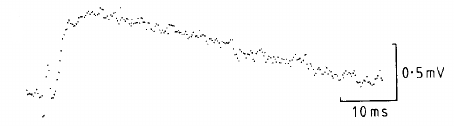
\includegraphics[scale=0.7]{PEPS}
	\caption{Potencial excitat�rio p�s sin�ptico recorrente em uma
             c�lula de Rewshaw \cite{walmsley81}.}
	\label{fig:PEPS}
\end{figure}

Para simular o experimento descrito, uma corrente suficiente para causar
um �nico potencial de a��o foi injetada no soma de um
MN do tipo S que fazia sinapse com uma CR. Para garantir uma atividade
passiva da membrana, a condut�ncia sin�ptica ativada pelo disparo do MN
foi diminu�da.

\subsubsection{Caracter�sticas de disparos}
Os par�metros de limiar, comprimento, di�metro e densidade e vari�veis de
transi��o das condut�ncias i�nicas do modelo da CR podem ser alterados
para reproduzir diferentes caracter�sticas de disparos. As altera��es feitas 
foram baseadas nas seguintes refer�ncias:

\begin{itemize}
    \item \citeonline{walmsley81}: Foi mostrado que CRs disparam
        espontaneamente a uma taxa de 7 pps.
    \item \citeonline{hultborn79}: Rela��es de frequ�ncia de disparo
        \textit{versus} corrente injetada ($\freq\times\iinj$) foram obtidas para 
        diferentes correntes, como visto na Figura
        \ref{fig:HP79}\subref{fig:fxiRC}. Nessas curvas, informa��es sobre
        a forma como a CR se adapta a uma dada corrente e a intensidade 
        de corrente necess�ria para que os disparos comecem a acontecer
        tamb�m podem ser extra�das. Al�m dessas contribui��es, os autores
        mostraram que, ap�s um breve pulso de corrente injetada,
        a AHP apresentou uma amplitude de -2 mV e dura��o por volta de 30 ms,
        como visto na Figura \ref{fig:HP79}\subref{fig:AHPRC}.
    \item \citeonline{fyffe90}: Estudos morfol�gicos mostraram CRs com 
        di�metro m�dio de de 27 $\mu$m.
    \item \citeonline{bui03}: Estimativas da �rea superficial m�dia do soma
        e do dendrito foram 1753.8 $\mu\text{m}^2$ e 16756 $\mu\text{m}^2$,
        respectivamente.
\end{itemize}

\begin{figure}[ht]
    \centering
    \subfloat[][]{
        \label{fig:fxiRC}
        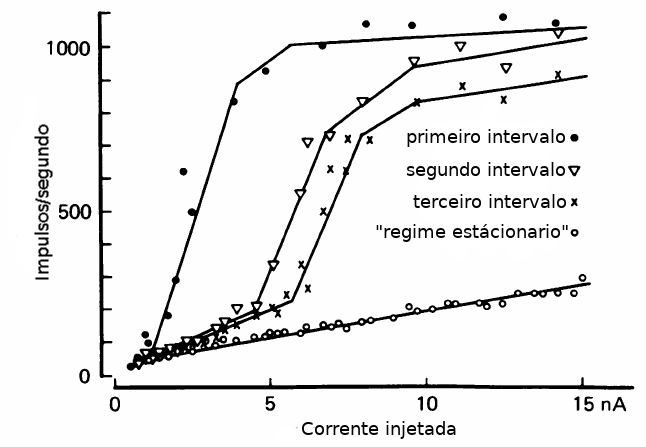
\includegraphics[scale=0.4]{fxiRC}
    }
    \hspace{-1cm}
    \subfloat[][]{
        \label{fig:AHPRC}
        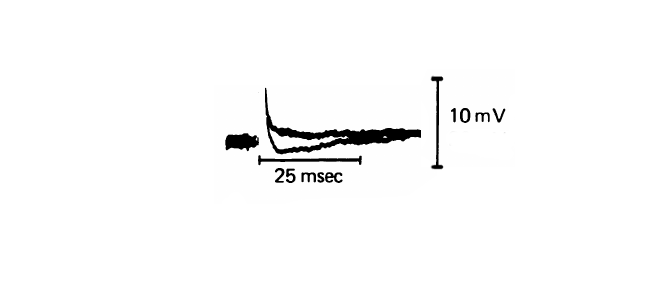
\includegraphics[scale=0.5]{AHPRC}
    }
    \caption[Caracter�sticas de disparos disparos da c�lula de Renshaw
            \cite{hultborn79}]{
        Caracter�sticas de disparos disparos da c�lula de Renshaw
        \cite{hultborn79}. \subref{fig:fxiRC} Rela��o entre corrente
        injetada e taxa de disparo de uma c�lula de Renshaw.
        A taxa de disparo instant�nea entre o primeiro e segundo potencial
        de a��o � entendido como o 
        primeiro intervalo, e assim por diante. O regime estacion�rio foi
        considerado como sendo ap�s 80 ms. 
        \subref{fig:AHPRC} Detalhes de
        amplitude e dura��o da p�s hiperpolariza��o.
}
    \label{fig:HP79}
\end{figure}

Primeiramente, � necess�rio definir quando a CR ir� disparar
um potencial de a��o. Sabe-se que esses neur�nios possuem
baixo limiar \cite{uchiyama03a}, mas n�o existem estudos quantitativos
especificamente sobre esse par�metro. O valor do limiar foi calculado como

\begin{equation}
\thresh=\frac{\rheo R_m}{\supArea}
\label{eq:vth}
\end{equation}

com $V_l$ sendo a tens�o de limiar, $I_r$ a corrente de reobase e $a$ a 
�rea superficial total \cite{cisi07}. Para calcular o comprimento \length de um
�nico compartimento, por sua vez, foi usada a express�o

\begin{equation}
    a=\pi ld
    \label{eq:area}
\end{equation}

sendo \diam o di�metro da CR \cite{sterratt11}.

A partir de ent�o, simula��es foram realizadas com diferentes valores de
vari�veis de transi��o e densidade das condut�ncias i�nicas de uma �nica CR
para se encontrar resultados de AHP e curva $F\times I$ apropriados. As correntes
injetadas em cada caso estiveram de acordo com os dados mostrados na Figura
\ref{fig:HP79}. Por fim, para obter uma taxa de disparos espont�neos de 7 pps,
foi necess�rio alterar o valor da condut�ncia m�xima do ru�do agindo sobre
a CR.

\subsubsection{Potenciais inibit�rios p�s sin�pticos}
As condut�ncias sin�pticas ativadas pelos disparos das CRs em cada
tipo de MN foram ajustadas, levando em conta os seguintes dados experimentais:

\begin{itemize}
    \item \citeonline{friedman81}: Correla��es foram encontradas entre
        amplitude dos PIPS e o tipo do MN, mas n�o entre amplitudes e 
        as resist�ncias de entrada dos MNs em cada tipo.
    \item \citeonline{fyffe91}: Conex�es sin�pticas identificadas como
        provenientes de CRs foram todas localizadas nos dendritos de MNs
        do tipo alfa.
    \item \citeonline{uchiyama03a}: Baseado em dados fisiol�gicos
        \cite{friedman81,hultborn88b,vankeulen79}, um procedimento para
        estimar PIPS nos MNs de um n�cleo motor foi adotado, tendo os 
        resultados mostrados na Figura \ref{fig:met_IPSP}.
\end{itemize}

\begin{figure}[ht]
	\center
	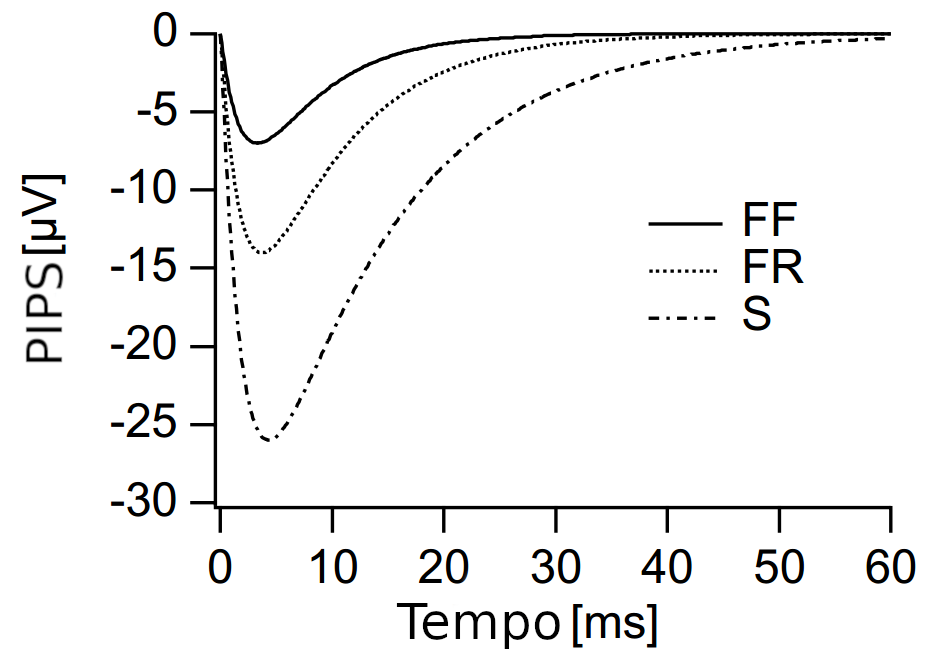
\includegraphics[scale=0.4]{met_IPSP}
    \caption[PIPS resultante agindo nos MNs]{
             PIPS resultante agindo nos MNs \cite{uchiyama03a}.
            }
	\label{fig:met_IPSP}
\end{figure}

Sendo assim, a localiza��o das sinapses das CRs foi definida no
compartimento dendr�tico do MN e simula��es foram realizadas para encontrar
tr�s valores de condut�ncias (um para cada tipo) que reproduzam a Figura 
\ref{fig:met_IPSP}.

\subsubsection{Distribui��o de potenciais inibit�rios p�s
                sin�pticos recorrentes}
                \label{sec:met_ipsp}
A distribui��o dos PIPS recorrentes pelo n�cleo motor depende 
de fatores topogr�ficos e funcionais. No ReMoto, isso est� relacionado
com condut�ncias sin�pticas e suas conex�es. Nas simula��es realizadas,
a conectividade entre MNs e CRs foi considerada como sendo de 
100\% e as condut�ncias e suas distribui��es topogr�ficas s�o parametrizadas
de acordo com:

\begin{itemize}
    \item \citeonline{mccurdy94}: A Distribui��o topogr�fica das amplitudes
        significativas de PIPS recorrentes obtida de pares de MNs �
        inversamente correlacionada com a dist�ncia. Os autores fornecem uma
        vis�o geral, independente do n�cleo motor. MNs do m�sculo gastrocn�mio
        medial separados por no m�ximo 1 mm s�o classificados como 
        pr�ximos. Fora dessa zona, s�o considerados distantes. A Figura
        \ref{fig:met_RIPSP} mostra o resultado dos autores. Para o m�sculo
        em quest�o, os valores m�dios de amplitudes foram de 
        -19,63 $\pm$ 2,42 $\mu$V e -41.36 $\pm$ 7.19 $\mu$V para pares
        distantes e pr�ximos, respectivamente.
    \item \citeonline{uchiyama03a}: O padr�o de distribui��o topogr�fica 
        da for�a sin�ptica � o de uma gaussiana que decresce na medida
        em que se afasta do neur�nio pr� sin�ptico. O desvio padr�o da
        curva � de 0.167 mm e 1.164 mm para os MNs e para as CRs, 
        respectivamente. A quantidade de bot�es sin�pticos tamb�m �
        um indicativo da for�a sin�ptica das conex�es. Estima-se que os
        ax�nios colaterais dos MNs que alcan�am a regi�o onde as CRs se
        encontram possuam 78.5 $\pm$ 7.5, 43.0 $\pm$ 4.2 e 35.5 $\pm$ 3
        destes bot�es sin�pticos se forem do tipo FF, FR e S, respectivamente.
\end{itemize}

\begin{figure}[ht]
	\center
	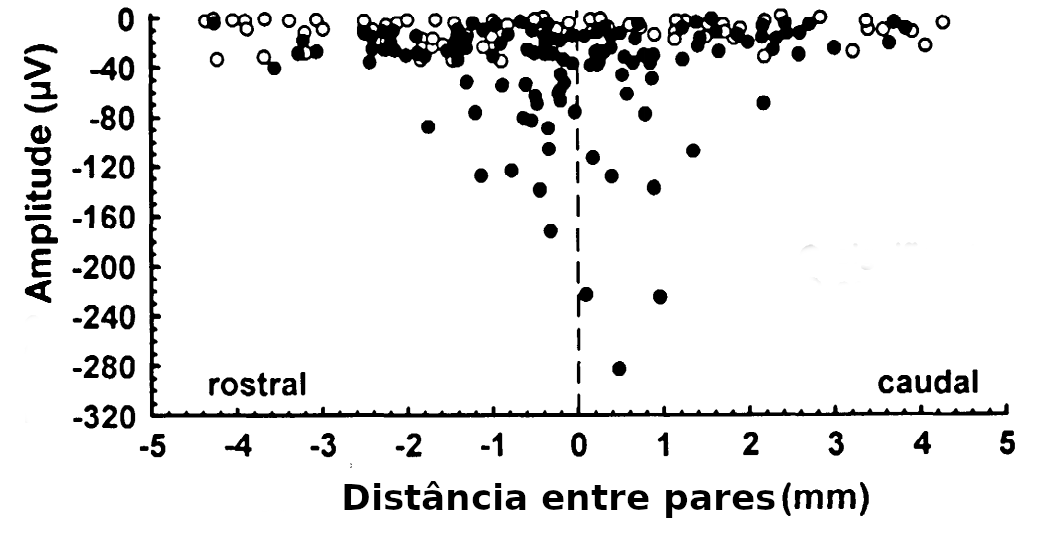
\includegraphics[scale=0.4]{met_RIPSP}
    \caption[Distribui��o topogr�fica de PIPS recorrentes]{
             Distribui��o topogr�fica de PIPS recorrentes. Valores
             na abcissa indicam a dist�ncia entre os pares de MNs
             enquanto que a ordenada mostra o valor da amplitude do 
             PIPS recorrente gerado. Pontos pretos e brancos representam as respostas
             significantes e as possivelmente equ�vocas, respectivamente
             \cite{mccurdy94}.}
	\label{fig:met_RIPSP}
\end{figure}

Para reproduzir o experimento como em \citeonline{mccurdy94}, as simula��es
consistiram em correntes injetadas no soma de MNs por um curto per�odo de 
tempo para que o PIPS recorrente pudesse ser observado em outros MNs.
Foram levados em conta 180 pares, separados por dist�ncias entre
86 $\mu$m e 4.7 mm. O n�mero de CRs, de acordo com as estimativas,
foi de 600.

O n�mero
de bot�es sin�pticos de cada tipo de MN nas CRs foi implementado como valores
de condut�ncia seguindo uma propor��o de 1:0.55:0.45 (FF:FR:S). Isso
permitiu que apenas a condut�ncia m�xima dos MNs do tipo FF
\gmaxff fosse parametrizado, sendo as outras ajustadas
de acordo com a propor��o.

\subsubsection{Din�mica e depress�o sin�ptica}
Para abordar as caracter�sticas din�micas e de depress�o p�s sin�ptica,
as refer�ncias utilizadas foram:

\begin{itemize}
    \item \citeonline{hultborn79}: Os autores apresentaram
          evid�ncias da exist�ncia de um mecanismo de decr�scimo da efic�cia
          sin�ptica dos terminais de ax�nios colaterais agindo sobre as CRs.
          Essa conclus�o foi baseada na diminui��o de taxas de disparo para
          diferentes frequ�ncias de est�mulo. 
    \item \citeonline{uchiyama03a}: Um aumento abrupto na frequ�ncia de
          estimula��o da CR fez com que sua
          taxa de disparo apresentasse um \textit{overshoot}, como
          mostrado na Figura \ref{fig:met_dyn}
\end{itemize}

\begin{figure}[ht]
	\center
	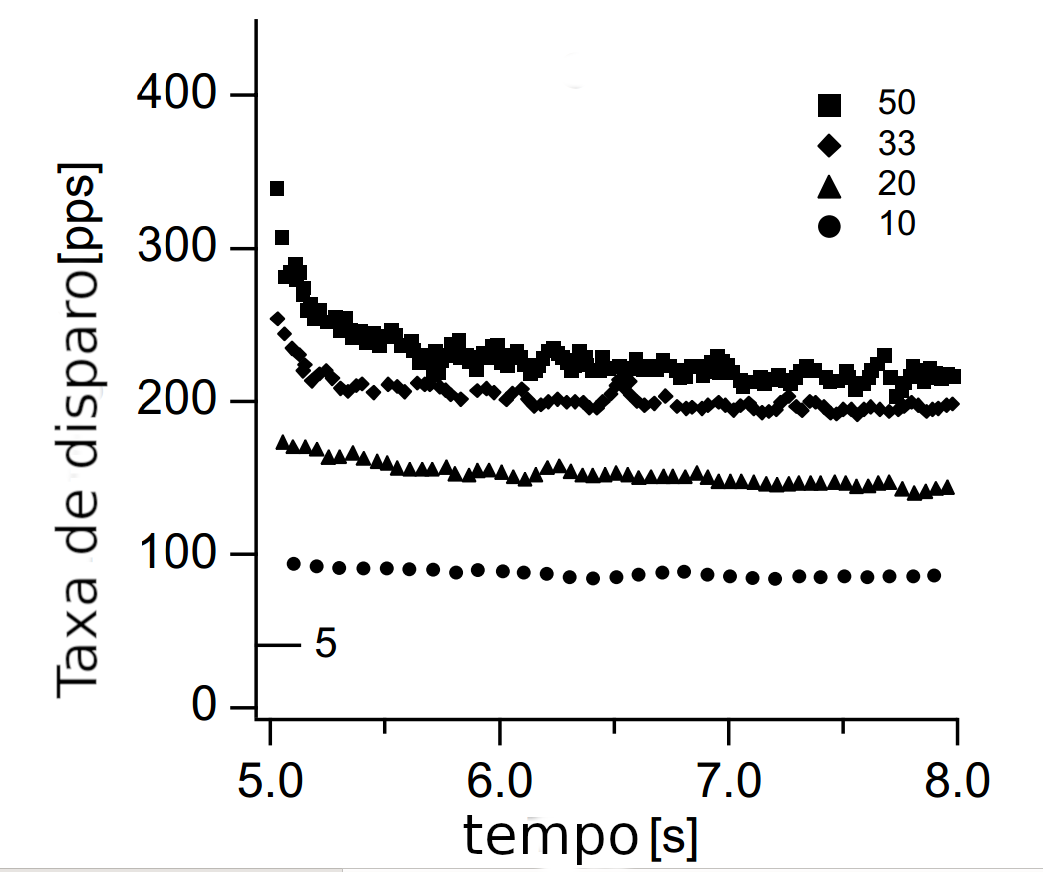
\includegraphics[scale=0.4]{met_dyn.png}
    \caption[Caracter�sticas din�micas da c�lula de Renshaw.]{
             Caracter�sticas din�micas da c�lula de Renshaw.
             A frequ�ncia do est�mulo
             aplicado, inicialmente
             de 5 Hz (com resposta indicada pelo tra�o horizontal com o
             n�mero 5 no eixo
             vertical), foi abruptamente aumentada para um dos valores
             indicados na legenda, em Hz \cite{uchiyama03a}.
            }
	\label{fig:met_dyn}
\end{figure}

No ReMoto, uma depress�o p�s sin�ptica em fun��o do tempo � descrita por

\begin{equation}
    \gsyn (t)=\gmax-(\gmax-g_{dyn}\vari)e^{-\frac{(\td+t)}{\tau}}
\end{equation}

sendo $g_{dyn}$ a condut�ncia din�mica alterada pela depress�o
ap�s um disparo, \gmax a condut�ncia m�xima original, \vari o 
quanto de depress�o ocorrer� ($0\le\vari\le 1$), $\tau$ a 
constante de tempo e $t_d$ o instante do �ltimo disparo.

As simula��es para ambas caracter�sticas foram feitas com uma 
popula��o de CRs recebendo um est�mulo antidr�mico
com frequ�ncias variadas para que a taxa de disparos gerada
fosse contabilizada.

\subsection{Valida��o do modelo}
Nesta se��o, de forma qualitativa e
semiquantitativa, a robustez da parametriza��o adotada foi testada por meio
da compara��o de resultados de procedimentos experimentais com resultados
obtidos da simula��o desses experimentos.

\subsubsection{Caracter�sticas de potenciais inibit�rios
            p�s sin�pticos recorrentes}
As caracter�sticas de PIPS recorrentes que foram verificadas 
s�o mostradas na Figura \ref{fig:met_hamm}. As simula��es realizadas 
foram as mesmas da parametriza��o na Se��o \ref{sec:met_ipsp}.

\begin{figure}[ht]
	\center
	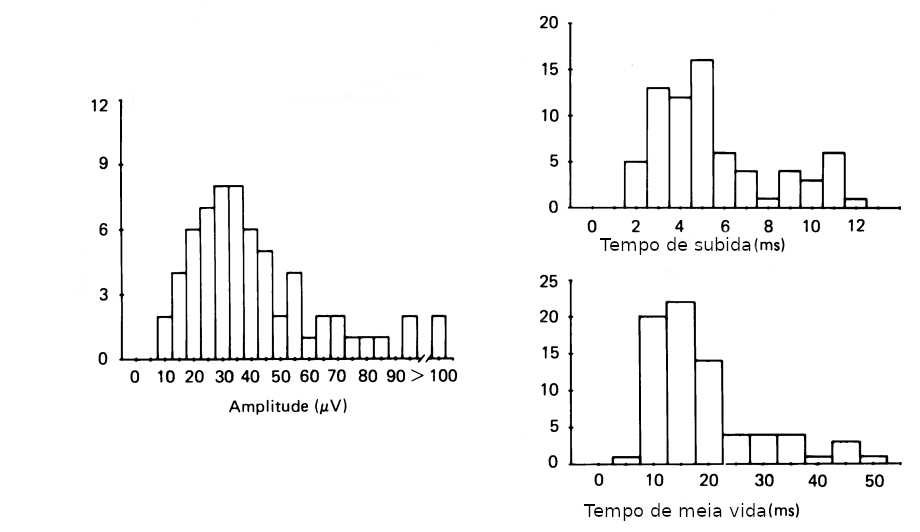
\includegraphics[scale=1.3]{met_hamm}
    \caption[Resultados experimentais sobre caracter�sticas de PIPS
            recorrentes.]{
            Resultados experimentais sobre caracter�sticas de PIPS
            recorrentes. Eixos verticais s�o as contagens de ocorr�ncias
            \cite{hamm87b}.}
	\label{fig:met_hamm}
\end{figure}

\subsubsection{Rela��o est�tica das entradas e sa�das das c�lulas de Renshaw}
A rela��o est�tica de entrada e sa�da realizada por \citeonline{cleveland81}
� importante para a caracteriza��o de CRs. Foi observado que os resultados
obtidos poderiam ser ajustados a uma fun��o hiperb�lica, que por
conveni�ncia foi chamada de fun��o de Langmuir pelos autores. Esta abordagem
tamb�m foi empregada nesse trabalho e a fun��o em quest�o foi calculada como

\begin{equation}
    \fcr=\frac{\satConst\fad}{\constSemiSat+f_{AD}}
\end{equation}

em que $f_{AD}$ � a frequ�ncia do est�mulo, $f_{CR}$ � a taxa de disparo
m�dia da CR ap�s sua resposta transiente,
$c$ � a constante de satura��o e $k$ � a 
constante de semissatura��o. Esta an�lise foi reproduzida
no modelo parametrizado, passado um per�odo de adapta��o do neur�nio 
de 500 ms e 
considerando as frequ�ncias de est�mulos antidr�micos como entrada e
taxas de disparos das CRs como sa�da. Os resultados experimentais
da literatura s�o
os mostrados na Figura \ref{fig:met_cleveland}

\begin{figure}[ht]
	\center
	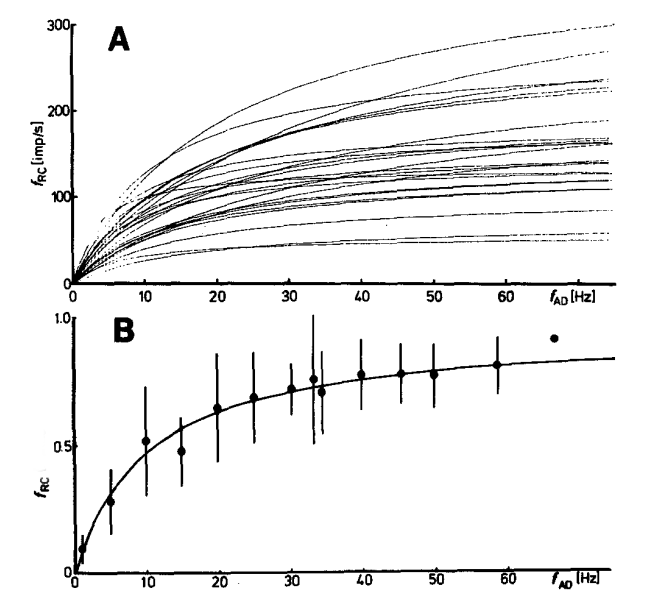
\includegraphics[scale=1.3]{met_cleveland}
    \caption[Resultados experimentais sobre rela��es est�ticas de 
            entrada e sa�da.]{
            Resultados experimentais sobre rela��es est�ticas de 
            entrada e sa�da. Uma frequ�ncia de est�mulo antidr�mica
            $f_{AD}$ em Hz gera uma taxa de disparos $f_{RC}$ na CR.
            No gr�fico superior, 24 fun��es de Langmuir s�o ajustadas
            �s respostas de 24 CRs. No gr�fico inferior, a m�dia
            normalizada desse grupo � apresentada, tamb�m com uma
            fun��o de Langmuir ajustada a ela. Barras verticais
            representam o desvio padr�o.
            \cite{cleveland81}.}
	\label{fig:met_cleveland}
\end{figure}

\subsubsection{Respostas das c�lulas de Renshaw sujeitas a um est�mulo
            antidr�mico}
As CRs, quando ativadas por todos os ax�nios motores convergindo
nelas, exibem disparos que podem durar at� algumas dezenas de
milissegundos e taxas de disparos
instant�neas decrescentes com o tempo e dependentes da for�a sin�ptica 
total \cite{eccles61b,uchiyama03a}. Essa caracter�stica � mostrada na 
Figura \ref{fig:met_eccles}

\begin{figure}[ht]
	\center
	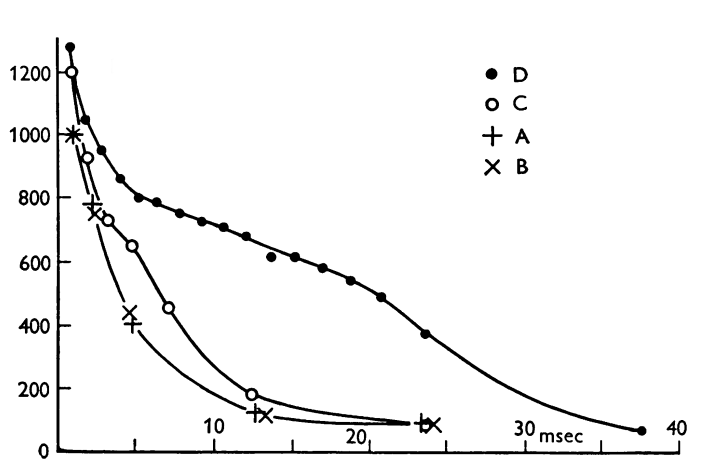
\includegraphics[scale=1.3]{met_eccles}
    \caption[CRs e sua resposta � um est�mulo antidr�mico.
            ]{CRs e sua resposta � um est�mulo antidr�mico.
            O tempo � mostrado na abcissa, em ms, enquanto
            que a taxa de disparos, na ordenada, em pps.
            S�o mostradas respostas de diferentes n�cleos 
            motores, de acordo com a legenda: A, plantar;
            B, s�leo; C, gastrocn�mio medial; D, gastrocn�mio
            lateral \cite{eccles61b}.}
	\label{fig:met_eccles}
\end{figure}

Nas simula��es realizadas, a atividade espont�nea das CRs foi ativada
e os est�mulos antidr�micos foram aplicados com diferentes intensidades
para ativar diferentes tipos de MNs. As taxas de disparos instant�neas
foram calculadas como o rec�proco do intervalo entre cada potencial de
a��o, em pps.

\section{Efeitos da parametriza��o em simula��es}
O objetivo desta etapa � entender como o modelo parametrizado se comporta 
em diferentes situa��es, algumas das quais se basearam em trabalhos
experimentais ou em outros computacionais. Dessa forma,
foram configuradas simula��es que eram o mais semelhantes poss�vel a esses 
trabalhos para que os resultados pudessem ser apropriadamente comparados.
De formal geral, todas as simula��es tiveram
CRs disparando espontaneamente.

\subsection{Disparos de motoneur�nios}
\label{sec:met_onion}
Com o intuito de analisar o recrutamento dos MNs,
uma corrente \injCur
em fun��o do tempo foi injetada no soma de todos esses neur�nios. Nessa
simula��o, a presen�a ou aus�ncia da inibi��o recorrente � analisada no
mesmo circuito e a corrente $i(t)$ � descrita pela seguinte equa��o:

\begin{equation}
    i(t)=40t/1000.
    \label{eq:i}
\end{equation}

Outra op��o utilizada para estimular os MNs foi com
uma entrada excitat�ria que aumenta com o tempo de simula��o,
mas, nesse caso, isso se d� por meio de
fibras descendentes com
frequ�ncia de disparos \fd dada por

\begin{equation}
FD(t)=1500t/1000.
    \label{eq:fd}
\end{equation}

Em outra situa��o,
para estudar a taxa de disparos dos MNs, a entrada utilizada
foi dada por

\begin{equation}
    FD(t)=
    \left\{
        \begin{aligned}
            &\frac{\cvmPerc}{4000}t,\quad t\le 4000 ms \\
            &\cvmPerc,\quad 4000<t<5000 ms \\
            &-\frac{\cvmPerc}{4000}(t-9000),\quad t\ge 5000 ms
        \end{aligned}
    \right.
    \label{eq:ramphold}
\end{equation}

sendo \cvmPerc o valor necess�rio para alcan�ar a porcentagem da CVM desejada.
Esta equa��o representa os disparos de fibras descendentes agindo sobre
o n�cleo motor com o intuito de realizar uma contra��o em rampa at� 70 \%
da CVM. Ap�s 1 segundo nesse valor, eles deca�ram com a mesma derivada.

Nas simula��es com inibi��o recorrente, \cvmPerc de 950 foi suficiente
para recrutar por volta de 240 MNs \cite{walmsley78} no pico da
Equa��o (\ref{eq:ramphold}). Para fazer com que
o n�vel de for�a muscular gerado nessa situa��o
se mantivesse na aus�ncia das CRs, o valor dessa vari�vel foi
diminu�do para 710.

As taxas de disparos foram calculadas por meio da convolu��o de
uma janela de Hann de 400 ms de largura e �rea unit�ria com
um trem de impulsos unit�rios representando os instantes de 
disparos dos MNs.

\subsection{Diminui��es dos n�veis de for�a}
O efeito do modelo de CR na for�a muscular foi estudado baseando-se
no trabalho de \citeonline{granit61}, que fizeram uma estimativa 
do quanto a inibi��o recorrente diminuiria a tens�o gerado pelo 
m�sculo s�leo do gato. Isso � mostrado na Figura \ref{fig:met_granit}

\begin{figure}[ht]
	\center
	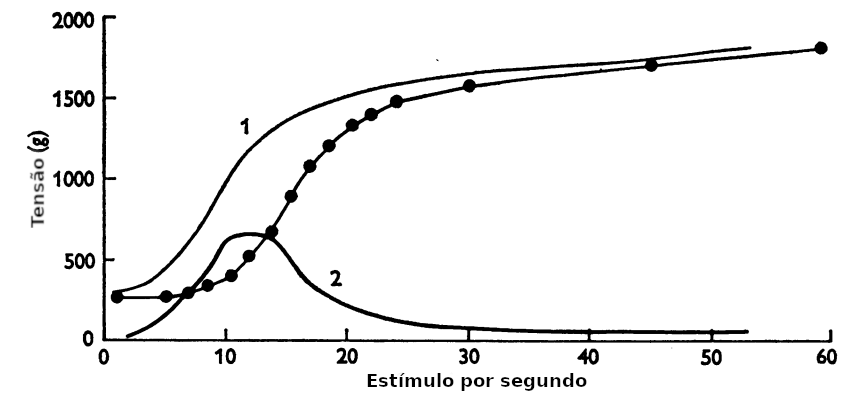
\includegraphics[scale=0.5]{met_granit}
    \caption[Tens�o isom�trica do m�sculo s�leo (ordenada) em fun��o
             da frequ�ncia de est�mulo do nervo (abcissa).]{
             Tens�o isom�trica do m�sculo s�leo (ordenada) em fun��o
             da frequ�ncia de est�mulo do nervo (abcissa). Os c�rculos
             preenchidos representam os valores de refer�ncia de tens�o
             muscular, enquanto que a curva 1 � uma estimativa dessa
             na aus�ncia de inibi��o recorrente. A curva 2 � a diferen�a
             das outras duas \cite{granit61}.}
	\label{fig:met_granit}
\end{figure}

Como o m�sculo utilizado nesse experimento � diferente do empregado
nas parametriza��es, algumas considera��es foram necess�rias.
Foi pressuposto que as rela��es dos MNs desse n�cleo motor
com as CRs e as fibras descendentes (condut�ncias sin�pticas e conectividade)
sejam as mesmas.
Ademais, as caracter�sticas de unidade motora relacionado aos 
\textit{twitches}, propriedades eletrot�nicas e geom�tricas foram as
mesmas adotadas para o n�cleo motor gastrocn�mio medial.
Dessa forma, apenas as quantidades e distribui��o de tamanhos
desses neur�nios foram alteradas, semelhante ao trabalho de
\citeonline{maltenfort98}.

A simula��o, portanto, foi realizada com
150 MNs do tipo S, de acordo com estimativas realizadas em trabalhos 
experimentais \cite{burke11}. Respeitando a propor��o de 50 MN/mm de medula
espinhal \cite{cisi07}, esses neur�nios foram distribu�dos
em 3 mm. Sendo assim, 300 CRs foram dispostos nesse comprimento
\cite{carr98}.
O n�cleo motor foi ativado por fibras descendentes durante 4 s,
com taxas suficientes para gerar os n�veis
de for�a reportados na Figura \ref{fig:met_granit}.

A m�dia da for�a em cada n�vel de estimula��o foi calculada,
descartando 1 s inicial que poderia conter respostas transit�rias.
Por estar diretamente
relacionada com a for�a gerada, a taxa de disparos m�dia dos MNs 
(computada como a m�dia das taxas individuais) e sua diminui��o 
causada pela inibi��o recorrente tamb�m foi analisada.

\subsection{An�lise espectral da for�a gerada pelo modelo}
\label{sec:met_psd}
Algumas condi��es simuladas por \citeonline{williams09},
como explicado  na se��o \ref{sec:intro_williams},
foram reproduzidas aqui para verificar se o modelo implementado no
ReMoto era capaz de reduzir oscila��es em 10 Hz.

Cada MN foi ativado por fibras descendentes com taxas de disparos
moduladas por
uma senoide com per�odo de 100 ms e valor m�dio suficiente para gerar
um n�vel de for�a desejado. Ru�dos excitat�rios
nos compartimentos dendr�ticos dos MNs foram adicionados
por meio de condut�ncias sin�pticas com valor de pico igual a 12 $\mu$S
ativadas por um processo pontual Poisson.
As frequ�ncias dessas duas entradas excitat�rias foram determinadas
como mostrado a seguir.

Primeiramente, usando o caso sem inibi�\~{a}o recorrente, a
frequ\^{e}ncia m�dia de disparo de fibras descendentes necess�ria 
para recrutar cerca de 75 MNs foi determinada. Essa quantidade
foi pr�xima de
25\% da popula��o de MNs ativados em n�veis de for�a de 5\% da CVM
\cite{hoffer87,walmsley78}. Por causa de fatores como conectividade e
propriedades dos MNs, algumas unidades motoras do tipo
FR foram ativadas. O mesmo procedimento foi realizado para n�veis
de 70\% da CVM, mas tendo a atividade de 80\% do n�cleo motor como
alvo \cite{hoffer87,walmsley78}.

Em seguida, para cada porcentagem da CVM adotada, foram considerados
cen�rios com inibi��o recorrente em que a condut�ncia das CRs
sob os MNs de cada tipo fosse igual, o dobro e a metade dos
respectivos valores apresentados na Tabela \ref{tab:params_final}.
Em cada um desses casos,
frequ�ncias m�dias de disparos foram ajustadas
para fazer com que as m\'{e}dias das for�as geradas estivessem
dentro de uma faixa de 10\% em torno da respectiva for�a gerada
na aus�ncia de CRs.

As frequ�ncias m�dias determinadas anteriormente foram utilizadas como valor
m�dio de uma senoide, que foi igual para todas as situa��es simuladas
nessa se��o. Sua amplitude pico a pico, determinada na situa��o
com condut�ncias das CRs inalteradas e com 5\% da CVM, 
foi aquela necess�ria para
fazer com que se fosse 
poss�vel observar picos no espectro da for�a e na coer�ncia
c�rtico-muscular parecidos com os de \citeonline{williams09}.

As caracter�sticas das fibras descendentes s�o
resumidas na Tabela
\ref{tab:met_dcistrat}. Em todos os cen�rios, a amplitude pico a pico
da senoide
foi de 4.6 Hz. Ademais, um ru�do independente com uma taxa pequena
de 90/s, suficiente para gerar cerca de 1/10 da condut�ncia total
causada pelas fibras descendentes no compartimento dendr�tico,
foi associado a todos os MNs.

\begin{table}[ht!]
\caption{Valores utilizados para as entradas nas simula��es em cada
    uma das situa��es estudadas.}
\label{tab:met_dcistrat}
\centering
    \begin{tabular}{c c c}\hline 
        \multirow{2}{*}{Situa��o da inibi��o recorrente} & \multicolumn{2}{c}{Frequ�ncias (Hz)} \\
             & \multicolumn{1}{c}{5\% CVM} & \multicolumn{1}{c}{70\% CVM} \\ \hline
        Ausente & 141 & 665 \\
        Fraca & 190 & 795 \\
        Normal & 230 & 930 \\
        Forte & 333 & 1180 \\
	\hline
    \end{tabular}
\end{table}

Uma outra condi��o simulada foi uma em que o valor m�dio da senoide
foi mantido o mesmo sem e com inibi��o recorrente.
Nesse caso, apenas a situa��o com 5\% da CVM e condut�ncias das CRs
inalteradas foi considerada.

A densidade espectral de pot�ncia da for�a muscular foi estimada por
meio do m�todo de 
Welch \cite{bendat11} com 5 janelas de Hann com 50\% de sobreposi��o.
A coer�ncia entre o sinal de EMG e o potencial de membrana do dendrito do MN de
�ndice 1, tomado como representativo da atividade neural descendente
oriunda do enc�falo, foi estimada
da mesma forma, mas com 33 janelas. O MN em quest�o recebia apenas
as entradas sin�pticas excitat�rias (potenciais de a��o de fibras
descendentes e ru�do), n�o era capaz de gerar potenciais de a��o 
e nem de fazer conex�es com CRs.

As simula��es realizadas tiveram dura��o de 11 s e passo de
integra��o de 0.05 ms. Para evitar
interfer�ncias de respostas transit�rias, apenas os �ltimos 
10 segundos dos sinais gerados pelo ReMoto foram utilizados.
As simula��es foram repetidas dez vezes
para que se fosse obtida uma resposta m�dia dos resultados, que 
foram, ent�o, comparadas qualitativamente com os resultados de
\citeonline{williams09} mostrados na Figura
\ref{fig:met_williams09}.

\begin{figure}[ht]
    \centering
    \subfloat[][]{
        \label{fig:met_williams09a}
        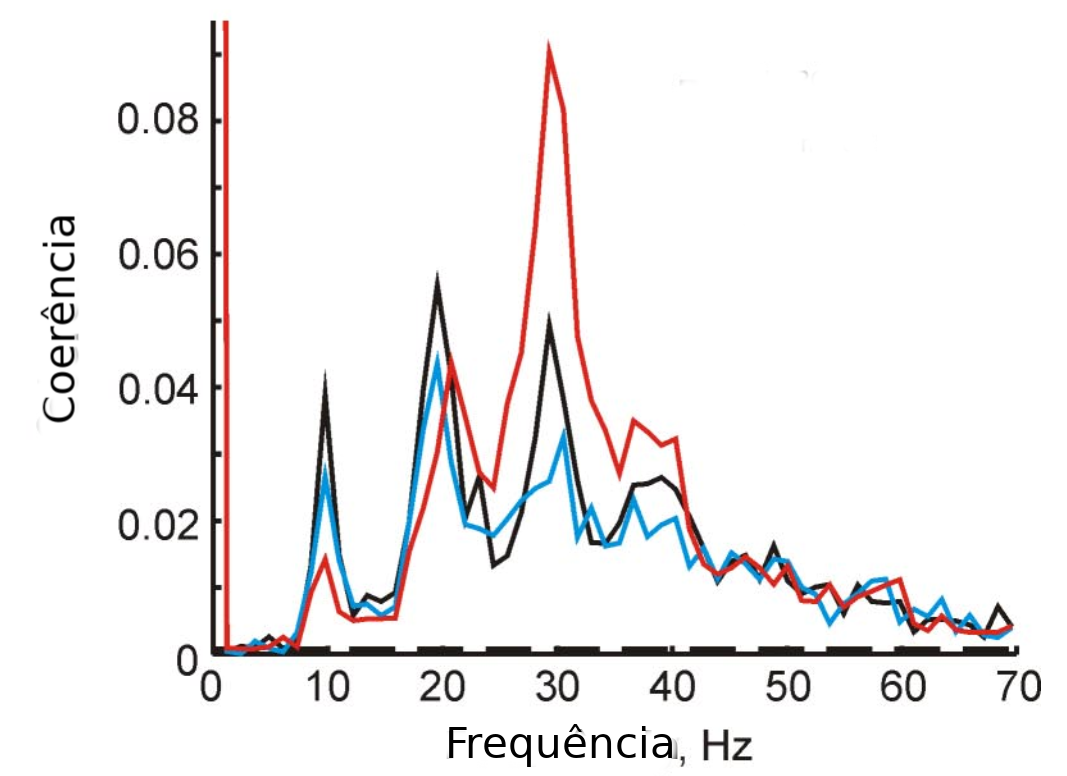
\includegraphics[scale=0.9]{met_williams09a}
    }
    \hspace{-1cm}
    \subfloat[][]{
        \label{fig:met_williams09b}
        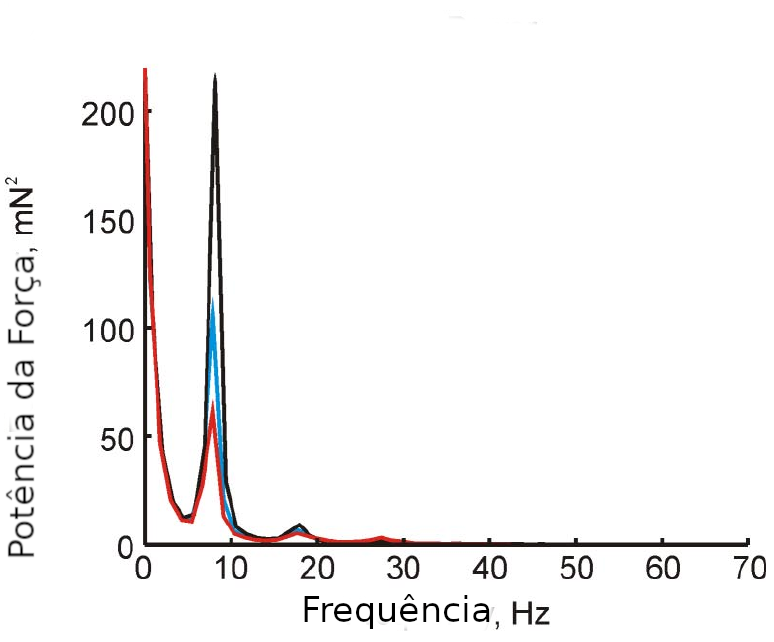
\includegraphics[scale=0.4]{met_williams09b}
    }
    \caption[Efeitos da aus�ncia e presen�a da c�lula de Renshaw em
            an�lises espectrais.]{Efeitos da aus�ncia e presen�a da
            c�lula de Renshaw an�lises espectrais.
            Linhas pretas e vermelhas
            s�o os resultados de simula��es sem e com CRs, respectivamente.
            A linha azul representa uma situa��o intermedi�ria e n�o ser�
            reproduzida aqui \cite{williams09}.
             \subref{fig:met_williams09a} Coer�ncia c�rtico-muscular.
             \subref{fig:met_williams09b} Espectro de pot�ncia da for�a muscular.
            }
	\label{fig:met_williams09}
\end{figure}

\subsection{Estudos de contra��es isom�tricas}
Os for�as de inibi��o recorrente e a forma como as entradas s�o
definidas para cada caso foram as mesmas das descritas na se��o 
anterior.
A ativa��o do n�cleo motor nessas simula��es foi
realizada por meio de fibras descendentes com taxa de disparos 
constantes e suficiente para gerar valores de for�a pr�ximos � CVM.
Essa taxa foi mantida por 500 ms.
Essa configura��o permitiu que a derivada da for�a, ou seja, sua 
sensibilidade ao comando descendente, pudesse ser avaliada para uma
situa��o de fuga de uma amea�a repentina.

Outros cen�rios analisados
foram os da manuten��o de 5\% e 70\% da CVM por meio de fibras
descendentes com taxas de disparo de potenciais de a��o constantes e 
suficientes para recrutar uma porcentagem de MNs pr�xima � apropriada
\cite{walmsley78}. Essas simula��es foram realizadas 10 vezes para cada
caso. O coeficiente de varia��o da for�a muscular 
gerada foi calculado pela equa��o (\ref{eq:cv}) mostrada abaixo:

\begin{equation}
    \text{Coeficiente de varia��o } (\%) = \frac{\text{desvio padr�o da for�a}}{\text{m�dia da for�a}}\cdot 100
    \label{eq:cv}
\end{equation}

Nesse caso, as simula��es tiveram dura��o de 2 s e os primeiros 500 ms 
foram removidos para evitar a presen�a de componentes transit�rios
no sinal.

Os cen�rios abordados na se��o \ref{sec:met_psd} tamb�m foram analisados aqui.
O valor das frequ�ncias de disparos foram
ajustados como na se��o \ref{sec:met_onion}. Em todos eles, os graus de 
sincronia foram calculados de acordo com o trabalho de
\citeonline{golomb01} e comparados.

O coeficiente de sincronia foi calculado da seguinte forma: Primeiramente,
a m�dia do potencial membrana do soma dos \numMN MNs que dispararam em uma simula��o 
foi dada como 

\begin{equation}
    \vMean(t) = \frac{1}{N}\sum_{i=1}^{N}\vInd(t)
\end{equation}

sendo sua vari�ncia calculada como 

\begin{equation}
    \statVar = \langle \vMean(t)^2\rangle_t - \langle \vMean(t)\rangle_t^2
\end{equation}

O operador $\langle\cdot\rangle_t$ denota uma m�dia no tempo. Em seguida, 
um fator de normaliza��o que leva em considera��o cada MN pode ser
calculado como 

\begin{equation}
    \sigma_i^2 = \langle V_i(t)^2\rangle_t - \langle V_i(t)\rangle_t^2
\end{equation}

Por fim, obt�m-se o coeficiente 

\begin{equation}
    \syncCoef = \frac{\sigma^2}{\frac{1}{N}\sum_{i=1}^N\sigma^2_i}
\end{equation}

em que $0\le\chi^2\le 1$. Sendo assim, valores mais pr�ximos de 1 indicam
uma atividade mais sincronizada do n�cleo motor.

\subsection{Distor��es na sa�da do n�cleo motor}
Nas simula��es descritas aqui, as entradas sin�pticas agindo sob o
n�cleo motor foram: Fibras descendentes com taxas de disparos com determinado
valor m�dio e moduladas por 3 senoides; ru�dos independentes
agindo sob cada MN. As senoides usadas para a modula��o tiveram frequ�ncias
de 0.5, 1 e 2.5 Hz, tendo amplitudes de 10, 5 e 2.5 Hz, respectivamente. O
ru�do, por sua vez, tiveram condut�ncia sin�ptica m�xima de 12 $\mu$S e 
e taxa de disparos de 50/s.

As simula��es envolveram
situa��es com e sem inibi��o recorrente. O valor m�dio da taxa de disparo
das fibras descendentes na aus�ncia das CRs foi ajustado para recrutar
cerca de 130 MNs. Em simula��es com CRs, o valor m�dio foi aumentado para
que fossem geradas for�as dentro de uma faixa de 10 \% em torno da for�a
gerada na situa��o anterior. Dessa forma, os valores utilizados foram de
300 e 438 Hz.

No total, foram realizadas 30 simula��es com 10 s de dura��o cada, sendo
os primeiros 2 s dos
sinais gerados removidos para eliminar poss�veis respostas transit�rias
nas an�lises subsequentes. A representa��o no dom�nio da frequ�ncia
da for�a muscular resultante foi obtida por meio da transformada de Fourier. 
Al�m disso, denominando \Bi como o pico do m�dulo da resposta em frequ�ncia em
0.5 ($i=1$), 1 ($i=2$) e 2.5 ($i=3$) Hz e \Bj como o das outras frequ�ncias,
os seguintes quantificadores foram calculados:

\begin{equation}
    \qum=\frac{B_1}{B_2}
    \label{eq:b1b2}
\end{equation}

\begin{equation}
    \qdois=\frac{B_1}{B_3}
    \label{eq:b1b3}
\end{equation}

\begin{equation}
    \qtres=\frac{\sqrt{B_1^2+B_2^2+B_3^2}}{\sqrt{\sum B_j^2}}
    \label{eq:pbipbni}
\end{equation}

Nessa �ltima express�o, a somat�ria foi realizada apenas at� as
componentes em frequ�ncia de 6 Hz. Para representar o sinal que � 
entregue aos m�sculos pelos MNs recrutados, foi utilizado um trem de disparos
cumulativo (CST, do ingl�s \textit{cumulative spike train}) filtrado
por um filtro passa-baixas de quarta ordem, do tipo \textit{Butterworth} e
com frequ�ncia de corte de 10 Hz.

	\chapter{Resultados Preliminares e Considera��es}
\section{Desempenho Computacional}
Na Figura \ref{fig:clustera} s�o apresentados os valores de \textit{speed up} das
simula��es com diferentes n�meros de processadores. Como se pode perceber, foi 
poss�vel alcan�ar uma diminui��o no tempo de execu��o com as simula��es feitas em
paralelo, de forma que os valores de \textit{speed up} aumentam de forma linear,
aproximadamente. Na Figura \ref{fig:clusterb}, por sua vez, s�o apresentados os valores das
efici�ncias calculadas. Esses valores s�o
bem pr�ximos para 2, 4 e 8 processos, mas uma queda come�a a se tornar vis�vel em
16 processos, sugerindo que, a partir desse n�mero, a queda de efici�ncia se 
acentue.

\begin{figure}[ht]
    \centering
    \subfloat[][]{
        \label{fig:clustera}
        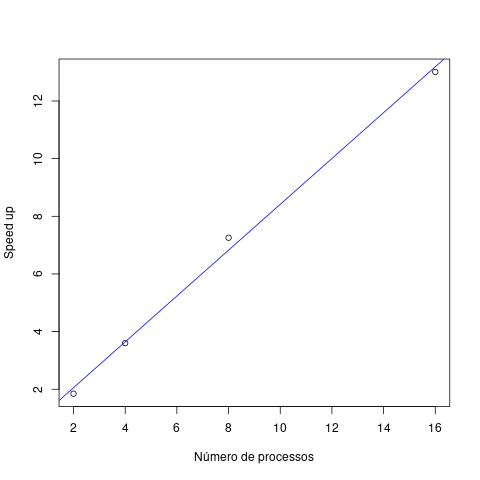
\includegraphics[scale=0.3]{linear}
    }
    ~ 
    \subfloat[][]{
        \label{fig:clusterb}
        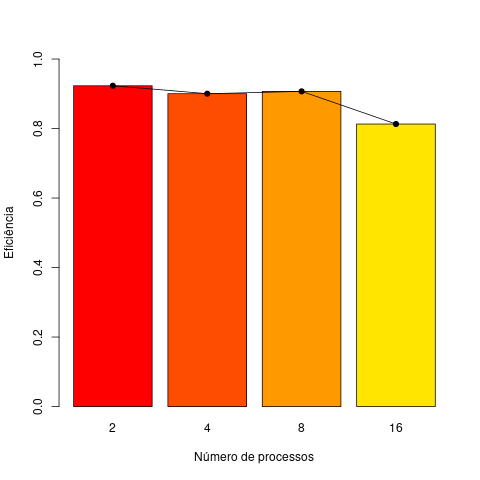
\includegraphics[scale=0.3]{efs}
    }
    \caption[Resultados de acelera��o e efici�ncia em fun��o do n�mero de processadores]{
        \subref{fig:clustera} Os c�rculos representam o \textit{speed up} obtido para cada
        n�mero de processador utilizado. A reta em azul mostra uma regress�o linear dos
        resultados. \subref{fig:clusterb} efici�ncia em fun��o do n�mero de processadores.
         }
\end{figure}

Outro resultado sobre desempenho computacional obtido foi o de tempo de
execu��o com as matrizes de condut�ncia alteradas no Python. Como mostrado na 
Tabela \ref{tab:matrixG}, n�o � observada uma melhora de desempenho quando se 
usa a $G_g$ para 10 MNs. Entretanto, a medida em que se aumentam
o n�mero de elementos neuronais para 50, 100 e 400 MNs, esta implementa��o
apresenta uma diminui��o do tempo de execu��o de aproximadamente 23\%, 29\% e
26\% em rela��o � $G_c$ com
10, 50, 100 e 400 MNs, respectivamente. Isso sugere que as otimiza��es trazidas
por essa estrat�gia s� s�o vantajosas para simula��es que envolvam $G_g$
relativamente grandes. Como essas matrizes s�o esparsas, algoritmos que se
aproveitam dessa estrutura podem ser usados para reduzir ainda mais o tempo de
simula��o.

\begin{table}[ht]
\caption{Tempo de execu��o das simula��es relacionadas 
         � matriz de condut�ncia para diferentes quantidades de MNs.}
\label{tab:matrixG}
\centering
    \begin{tabular}{ccccc}\hline 
        & 10 MNs & 50 MNs & 100 MNs & 400 MNs \\ \hline 
        $G_c$ & 5.21 s & 21.22 s & 42.34 s & 170.97 s \\ 
        $G_g$ & 5.63 s & 16.50 s & 30.01 s & 125.31 s \\ 
	\hline
    \end{tabular}
\end{table}

Os resultados mostrados anteriormente s�o positivos, mas possuem muitas
limita��es. Em primeiro lugar, apesar das melhoras obtidas com a matriz
$G_g$, a diferen�a de tempo de execu��o entre as vers�es Java e Python
ainda s�o muito grandes e outras solu��es precisariam ser exploradas
para diminuir essa discrep�ncia.

Em segundo lugar, � preciso enfatizar que os MNs das simula��es
realizadas no \textit{cluster} n�o recebem nenhuma entrada sin�ptica
de INs. A paraleliza��o desse tipo de configura��o �
facilmente obtida e dificilmente apresenta resultados negativos, pois,
como as unidades motoras s�o independentes umas das outras, os
processos podem executar em paralelo sem a necessidade de se comunicar. 
Em um cen�rio mais realista, como o que est� sendo estudado na Figura
\ref{fig:circuit}, MNs em um processo podem precisar receber informa��es
geradas em outro. Por causa da alta complexidade de conex�es
sinapticas, seriam necess�rias muitas comunica��es entre processos
e isso poderia causar uma diminui��o significativa nos valores de
\textit{speed up}.

Isso, de qualquer forma, n�o tira a validade desse resultado, visto
que existem maneiras de paralelizar simuladores de redes neuronais
complexas mantendo um bom desempenho computacional \cite{morrison05}.
Entretanto, pode-se perceber que os resultados obtidos no \textit{cluster},
em ess�ncia, poderiam ser reproduzidos em computadores comuns por meio
da utiliza��o de \textit{threads} ou processos. O uso destas estrat�gias,
na verdade, seria prefer�vel � utiliza��o de um \textit{cluster}, pois
envolvem menos altera��es na estrutura do c�digo do simulador e
possibilitam que outras pessoas interessadas em utilizar esse
\textit{software} possam fazer simula��es com um bom desempenho
computacional em seus pr�prios computadores.

A utiliza��o de \textit{threads} no Python, entretanto, n�o �
poss�vel por causa do \textit{Global Interpreter Lock} (GIL). Esse
mecanismo faz com que apenas uma \textit{thread} exista por processo.
Uma alternativa para essa limita��o � o uso de processos para realizar
a paraleliza��o do c�digo. Esse recurso pode ser explorado no Python
atrav�s da biblioteca \textit{Multiprocessing} e pode trazer melhoras
significativas, especialmente quando h� a possibilidade de se trabalhar
com mem�ria compartilhada. O c�digo do simulador, no entanto, teria que
passar por grandes modifica��es e sua estrutura de orienta��o a objetos
n�o � muito compat�vel com essa biblioteca. Al�m disso, a elevado 
volume de comunica��es entre processos aqui tamb�m seria um gargalo.

Sendo assim, de acordo com as observa��es feitas, conv�m propor outras
estrat�gias para alcan�ar um aumento no desempenho computacional. Para
esse fim, o Cython surge como uma boa alternativa e ser� explorado 
nesse trabalho, j� que seu uso pode ocasionar em tempos de execu��o
muitas vezes similares ao de um c�digo escrito em C \cite{gorelick14}.
Vale notar que o uso de \textit{clusters} ainda seria uma boa solu��o,
mas por causa da dificuldade de tal implementa��o e da exist�ncia de
outras op��es, esta � postergada para trabalhos futuros.

%\begin{table}[ht!]
%\caption{Tempo de execu��o das simula��es relacionadas 
%         � matriz de condut�ncia para diferentes tempos simulados.}
%\label{tab:matrixGt}
%\centering
%    \begin{tabular}{cccc}\hline 
%        & 200 ms & 500 ms & 1000 ms \\ \hline 
%        $G_c$ & 21.52 s & 53.03129 s &  s \\ 
%        $G_g$ & 16.55 s & 41.15 s &  s \\ 
%	\hline
%    \end{tabular}
%\end{table}

\section{Disparos dos Elementos Neuronais}
Na Figura \ref{fig:spkOldxNew}, cada MN � representado por �ndices, que 
s�o distribu�dos em ordem crescente no eixo vertical da figura e atribu�dos de
forma que seus valores sejam diretamente proporcionais ao tamanho dos
neur�nios aos quais est�o associados. O eixo horizontal representa os instantes
de disparo, que podem ser observados para cada �ndice. 

Pode-se perceber que o uso das
parametriza��es nova e antiga resulta em padr�es de disparos claramente
distintos. Na nova, os MNs disparam de forma ordenada, do menor para o maior 
(com algumas pequenas varia��es).
Por outro lado, na antiga, a alta inibi��o das CRs nos MNs faz com que
alguns destes, em certos instantes, atrasem seus disparos. Como resultado, o
gr�fico dos instantes de disparos, nesse caso, possui um aspecto ``fragmentado''.

\begin{figure}[ht]
	\center
	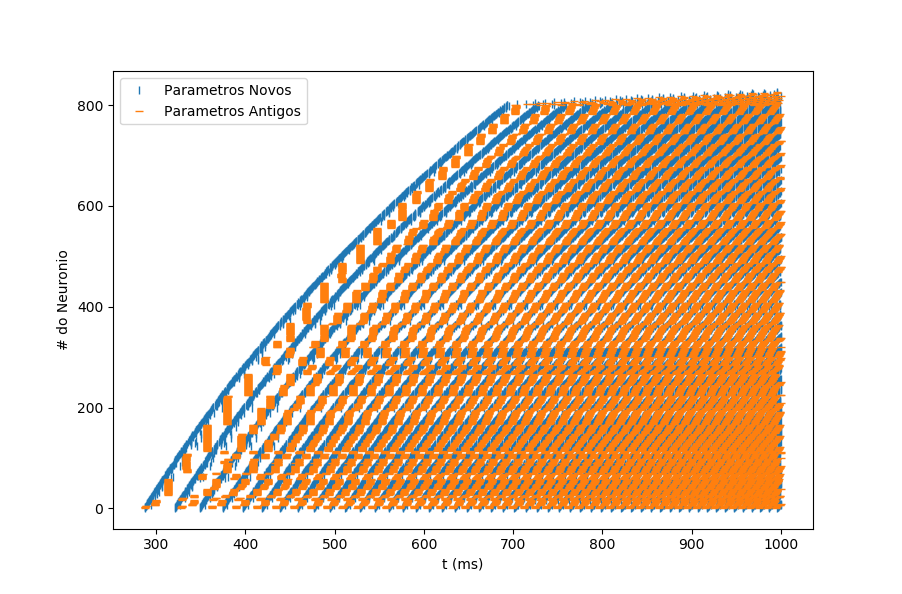
\includegraphics[scale=0.4]{spkOldxNew.png}
    \caption[Momentos de disparo dos somas de todos os motoneur�nios simulados.]{
             Momentos de disparo dos somas de todos os motoneur�nios simulados.
             O eixo das ordenadas representa os MNs e o eixo das abcissas, os
             instantes de disparo. Os disparos dos MNs, com
             parametriza��o nova e antiga das CRs, est�o sobrepostos.
            }
	\label{fig:spkOldxNew}
\end{figure}

Essa caracter�stica dos instantes de disparos usando a parametriza��o antiga
pode ser melhor observado na Figura 
\ref{fig:spkTimes}. � poss�vel perceber na Figura
\ref{fig:spkTimes}\subref{fig:spkOldZoom1} que algumas unidades com �ndice 
pr�ximo a 25 dispararam em 340 ms. Por volta de 25 ms antes, unidades com
�ndice perto de 60 j� tinham disparado. Na Figura
\ref{fig:spkTimes}\subref{fig:spkOldZoom2}, pode-se perceber que uma unidade
do tipo FR, de �ndice 801, dispara mais de 60 ms antes do que a do �ndice
anterior, que � do tipo S. Dessa forma, esses gr�ficos indicam que ocorreu
uma certa invers�o na ordem de recrutamento.

\begin{figure}[ht]
    \centering
    \subfloat[][]{
        \label{fig:spkOldZoom1}
        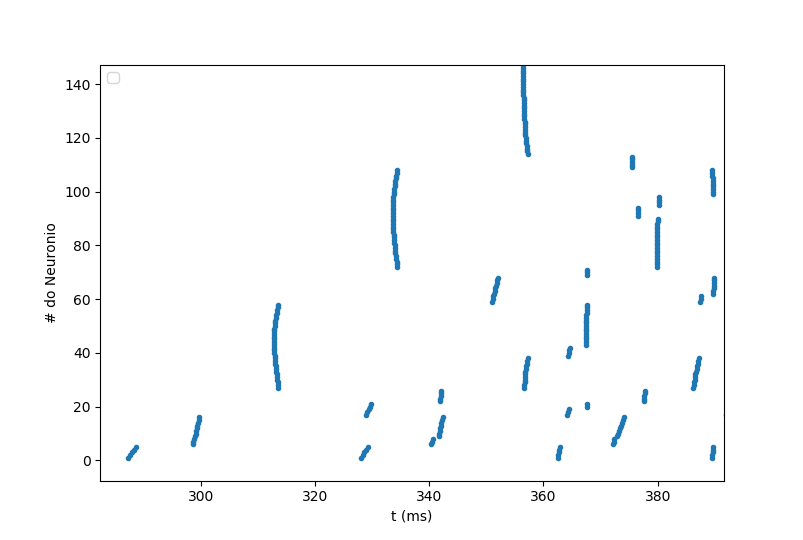
\includegraphics[scale=0.275]{spkOldZoom1.png}
    }
    ~ 
    \subfloat[][]{
        \label{fig:spkOldZoom2}
        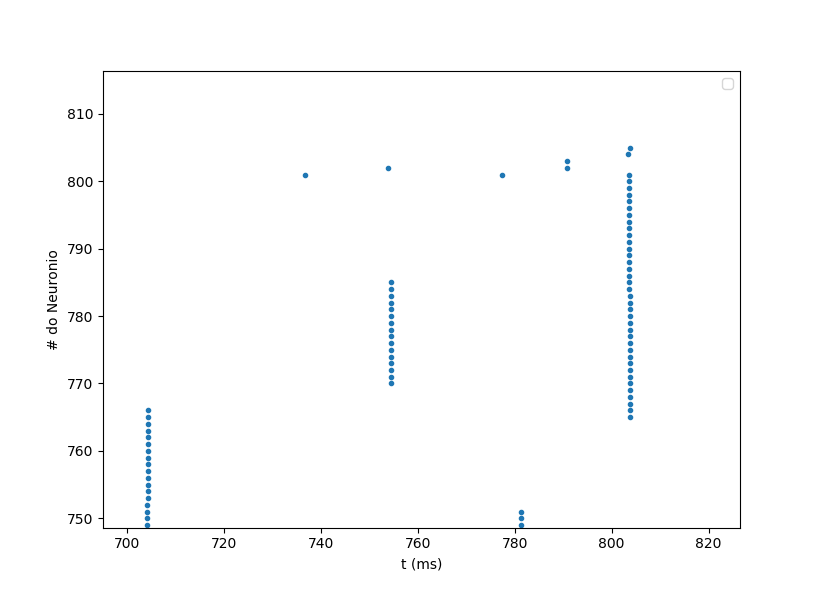
\includegraphics[scale=0.25]{spkOldZoom2.png}
    }
    \caption[Vis�o de um intervalo reduzido dos disparos dos motoneur�nios na
             parametriza��o antiga.]{
             Vis�o de um intervalo reduzido dos disparos dos motoneur�nios na 
             parametriza��o antiga.
             \subref{fig:spkOldZoom1} Instantes de disparos dos primeiros
             motoneur�nios nos instantes iniciais. \subref{fig:spkOldZoom2}
             Instantes de disparos dos �ltimos motoneur�nios nos instantes
             finais.
         }
    \label{fig:spkTimes}
\end{figure}

Para verificar se a for�a inibit�ria das CRs poderiam estar causando esse
comportamento, apenas os valores das condut�ncias entre CRs e MNs da
parametriza��o antiga foram substitu�dos por aqueles descrito em
\citeonline{maltenfort98}. O resultado dessa simula��o � mostrado 
na Figura \ref{fig:spkMaltenfort}\subref{fig:spkOldMaltenfort}. A apar�ncia
fragmentada dos disparos de MNs aparentemente desapareceu, mas
uma vis�o de um intervalo de tempo reduzido, como o da Figura
\ref{fig:spkMaltenfort}\subref{fig:spkOldMaltenfortZoom}, mostra que
o padr�o se tornou menos evidente. Esse resultado, no entanto, deixa em aberto
como que as CRs est�o influenciado os MNs, sendo necess�rio realizar
novamente algumas valida��es do circuito de inibi��o recorrente.

\begin{figure}[ht]
    \centering
    \subfloat[][]{
        \label{fig:spkOldMaltenfort}
        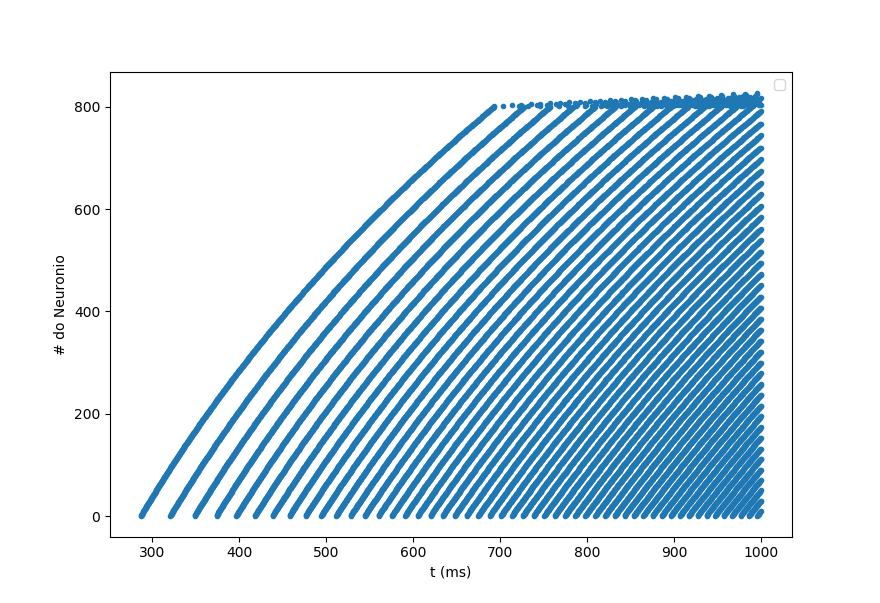
\includegraphics[scale=0.25]{spkOldMaltenfort.png}
    }
    ~ 
    \subfloat[][]{
        \label{fig:spkOldMaltenfortZoom}
        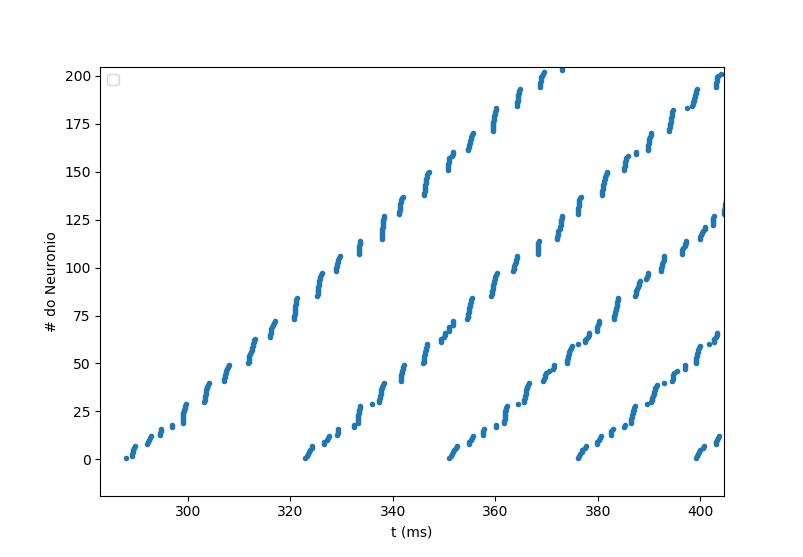
\includegraphics[scale=0.275]{spkOldMaltenfortZoom.png}
    }
    \caption[Momentos de disparo dos somas de todos os motoneur�nios
             simulados com as condut�ncias reportadas por
             \citeonline{maltenfort98}.]{Momentos de disparo dos somas
             de todos os motoneur�nios simulados com as condut�ncias
             reportadas por
             \citeonline{maltenfort98}. \subref{fig:spkOldMaltenfort} Vis�o 
             geral. \subref{fig:spkOldMaltenfortZoom} 
             Vis�o dos disparos em um intervalo reduzido.
         }
    \label{fig:spkMaltenfort}
\end{figure}

	%\include{sections/discussao}
	%\chapter{Conclus�es}
Os resultados relativos ao desempenho computacional apontam poss�veis
melhorias para o ReMoto.
A implementa��o de matrizes de condut�ncias adequada para opera��es
vetorizadas foi, inclusive, incorporada na vers�o do ReMoto em 
Fortran. A utiliza��o de \textit{clusters}, por sua vez, seria mais
complexa, envolvendo o desenvolvimento de uma arquitetura de processamento
que inclu�sse INs.

Baseando-se em dados experimentais, par�metros de MNs e CRs foram
ajustados para simular caracter�sticas importantes do circuito de
inibi��o recorrente. A parametriza��o foi satisfat�ria e foi poss�vel
observar uma s�rie de respostas apropriadas. Caracter�sticas din�micas
e de depress�o p�s-sin�ptica n�o puderam ser
reproduzidas como na literatura, mas essa limita��o, quando relevante,
foi considerada nas an�lises dos resultados de simula��es.

Para testar a parametriza��o adotada, simula��es de procedimentos
experimentais tamb�m foram realizadas. Rela��es est�ticas das CRs,
PIPS recorrentes e resposta a est�mulos antidr�micos do modelo foram
comparados com a literatura e utilizados
para delimitar propriedades gerais do modelo do circuito de inibi��o
recorrente gerado.

Considerando o que foi apresentado nos dois par�grafos anteriores,
pode-se dizer que o modelo parametrizado foi suficiente para os estudos 
aqui realizados sobre o circuito de inibi��o recorrente no gato.
Diferentemente
de outros trabalhos computacionais sobre as CRs, esse modelo foi
implementado em uma sistema de simula��o \textit{open source},
refor�ando aspectos importantes como extensibilidade e reproduzibilidade.

Considerando as parametriza��es realizadas,
resultados de simula��es sem e com inibi��o recorrente foram
avaliados sob diversas perspectivas. Os MNs sob efeito das CRs apresentaram
maior tend�ncia a inverter a ordem de seus recrutamentos,
algo que parece ter um efeito sobre a velocidade do desenvolvimento da
for�a muscular. Coeficientes de sincronia e de varia��o da for�a 
muscular tamb�m foram calculados, mas estudos experimentais s�o
necess�rios para esclarecer seus significados.

Diminui��es da for�a muscular foram compar�veis aos dados dispon�veis
na literatura. Al�m disso, an�lises no dom�nio da frequ�ncia mostraram
que as CRs poderiam atuar como um filtro passa baixas, atenuar oscila��es
de 10 Hz por meio de cancelamento de fases e causar distor��es.

Foi observado tamb�m que,
nas compara��es com aproximadamente o mesmo n�vel de for�a,
a presen�a das CRs causou diminui��es das taxas
de disparos, que foram acompanhadas por um aumento nas unidades motoras
recrutadas. O efeito das CRs nos CSTs, por sua vez, foi diferente
dependendo de quais MNs fossem escolhidos para realizar as computa��es.
Tais resultados refor�am a ideia de que a inibi��o recorrente seja
um mecanismo importante para o controle motor.

	
	\ProximoForaDoSumario
	\bibliography{library}
	\setboolean{ABNTNextOutOfTOC}{false}
	
	\apendice
	
	\chapter{Ap�ndice}

\index{ap�ndice}
Este cap�tulo � um Ap�ndice da Tese. Ap�ndices s�o cap�tulos com conte�do criado pelo autor, mas que n�o faz parte do tema central da Tese/Disserta��o.
	
	
	\anexo	
	\chapter{Anexo}


\index{anexo}
Este cap�tulo � um Anexo da Tese. Anexos s�o cap�tulos com conte�do que n�o foi criado pelo autor da Tese/Disserta��o.
	\setboolean{ABNTNextOutOfTOC}{false}
  
  \printindex
	
	
\end{document}

